% Options for packages loaded elsewhere
\PassOptionsToPackage{unicode}{hyperref}
\PassOptionsToPackage{hyphens}{url}
%
\documentclass[
]{book}
\usepackage{lmodern}
\usepackage{amssymb,amsmath}
\usepackage{ifxetex,ifluatex}
\ifnum 0\ifxetex 1\fi\ifluatex 1\fi=0 % if pdftex
  \usepackage[T1]{fontenc}
  \usepackage[utf8]{inputenc}
  \usepackage{textcomp} % provide euro and other symbols
\else % if luatex or xetex
  \usepackage{unicode-math}
  \defaultfontfeatures{Scale=MatchLowercase}
  \defaultfontfeatures[\rmfamily]{Ligatures=TeX,Scale=1}
\fi
% Use upquote if available, for straight quotes in verbatim environments
\IfFileExists{upquote.sty}{\usepackage{upquote}}{}
\IfFileExists{microtype.sty}{% use microtype if available
  \usepackage[]{microtype}
  \UseMicrotypeSet[protrusion]{basicmath} % disable protrusion for tt fonts
}{}
\makeatletter
\@ifundefined{KOMAClassName}{% if non-KOMA class
  \IfFileExists{parskip.sty}{%
    \usepackage{parskip}
  }{% else
    \setlength{\parindent}{0pt}
    \setlength{\parskip}{6pt plus 2pt minus 1pt}}
}{% if KOMA class
  \KOMAoptions{parskip=half}}
\makeatother
\usepackage{xcolor}
\IfFileExists{xurl.sty}{\usepackage{xurl}}{} % add URL line breaks if available
\IfFileExists{bookmark.sty}{\usepackage{bookmark}}{\usepackage{hyperref}}
\hypersetup{
  pdftitle={Quantitative Forschung in HRM: Eine methodische Einführung},
  pdfauthor={Dominik E. Froehlich},
  hidelinks,
  pdfcreator={LaTeX via pandoc}}
\urlstyle{same} % disable monospaced font for URLs
\usepackage{color}
\usepackage{fancyvrb}
\newcommand{\VerbBar}{|}
\newcommand{\VERB}{\Verb[commandchars=\\\{\}]}
\DefineVerbatimEnvironment{Highlighting}{Verbatim}{commandchars=\\\{\}}
% Add ',fontsize=\small' for more characters per line
\usepackage{framed}
\definecolor{shadecolor}{RGB}{248,248,248}
\newenvironment{Shaded}{\begin{snugshade}}{\end{snugshade}}
\newcommand{\AlertTok}[1]{\textcolor[rgb]{0.94,0.16,0.16}{#1}}
\newcommand{\AnnotationTok}[1]{\textcolor[rgb]{0.56,0.35,0.01}{\textbf{\textit{#1}}}}
\newcommand{\AttributeTok}[1]{\textcolor[rgb]{0.77,0.63,0.00}{#1}}
\newcommand{\BaseNTok}[1]{\textcolor[rgb]{0.00,0.00,0.81}{#1}}
\newcommand{\BuiltInTok}[1]{#1}
\newcommand{\CharTok}[1]{\textcolor[rgb]{0.31,0.60,0.02}{#1}}
\newcommand{\CommentTok}[1]{\textcolor[rgb]{0.56,0.35,0.01}{\textit{#1}}}
\newcommand{\CommentVarTok}[1]{\textcolor[rgb]{0.56,0.35,0.01}{\textbf{\textit{#1}}}}
\newcommand{\ConstantTok}[1]{\textcolor[rgb]{0.00,0.00,0.00}{#1}}
\newcommand{\ControlFlowTok}[1]{\textcolor[rgb]{0.13,0.29,0.53}{\textbf{#1}}}
\newcommand{\DataTypeTok}[1]{\textcolor[rgb]{0.13,0.29,0.53}{#1}}
\newcommand{\DecValTok}[1]{\textcolor[rgb]{0.00,0.00,0.81}{#1}}
\newcommand{\DocumentationTok}[1]{\textcolor[rgb]{0.56,0.35,0.01}{\textbf{\textit{#1}}}}
\newcommand{\ErrorTok}[1]{\textcolor[rgb]{0.64,0.00,0.00}{\textbf{#1}}}
\newcommand{\ExtensionTok}[1]{#1}
\newcommand{\FloatTok}[1]{\textcolor[rgb]{0.00,0.00,0.81}{#1}}
\newcommand{\FunctionTok}[1]{\textcolor[rgb]{0.00,0.00,0.00}{#1}}
\newcommand{\ImportTok}[1]{#1}
\newcommand{\InformationTok}[1]{\textcolor[rgb]{0.56,0.35,0.01}{\textbf{\textit{#1}}}}
\newcommand{\KeywordTok}[1]{\textcolor[rgb]{0.13,0.29,0.53}{\textbf{#1}}}
\newcommand{\NormalTok}[1]{#1}
\newcommand{\OperatorTok}[1]{\textcolor[rgb]{0.81,0.36,0.00}{\textbf{#1}}}
\newcommand{\OtherTok}[1]{\textcolor[rgb]{0.56,0.35,0.01}{#1}}
\newcommand{\PreprocessorTok}[1]{\textcolor[rgb]{0.56,0.35,0.01}{\textit{#1}}}
\newcommand{\RegionMarkerTok}[1]{#1}
\newcommand{\SpecialCharTok}[1]{\textcolor[rgb]{0.00,0.00,0.00}{#1}}
\newcommand{\SpecialStringTok}[1]{\textcolor[rgb]{0.31,0.60,0.02}{#1}}
\newcommand{\StringTok}[1]{\textcolor[rgb]{0.31,0.60,0.02}{#1}}
\newcommand{\VariableTok}[1]{\textcolor[rgb]{0.00,0.00,0.00}{#1}}
\newcommand{\VerbatimStringTok}[1]{\textcolor[rgb]{0.31,0.60,0.02}{#1}}
\newcommand{\WarningTok}[1]{\textcolor[rgb]{0.56,0.35,0.01}{\textbf{\textit{#1}}}}
\usepackage{longtable,booktabs}
% Correct order of tables after \paragraph or \subparagraph
\usepackage{etoolbox}
\makeatletter
\patchcmd\longtable{\par}{\if@noskipsec\mbox{}\fi\par}{}{}
\makeatother
% Allow footnotes in longtable head/foot
\IfFileExists{footnotehyper.sty}{\usepackage{footnotehyper}}{\usepackage{footnote}}
\makesavenoteenv{longtable}
\usepackage{graphicx,grffile}
\makeatletter
\def\maxwidth{\ifdim\Gin@nat@width>\linewidth\linewidth\else\Gin@nat@width\fi}
\def\maxheight{\ifdim\Gin@nat@height>\textheight\textheight\else\Gin@nat@height\fi}
\makeatother
% Scale images if necessary, so that they will not overflow the page
% margins by default, and it is still possible to overwrite the defaults
% using explicit options in \includegraphics[width, height, ...]{}
\setkeys{Gin}{width=\maxwidth,height=\maxheight,keepaspectratio}
% Set default figure placement to htbp
\makeatletter
\def\fps@figure{htbp}
\makeatother
\setlength{\emergencystretch}{3em} % prevent overfull lines
\providecommand{\tightlist}{%
  \setlength{\itemsep}{0pt}\setlength{\parskip}{0pt}}
\setcounter{secnumdepth}{5}

\title{Quantitative Forschung in HRM: Eine methodische Einführung}
\author{Dominik E. Froehlich}
\date{2020}

\begin{document}
\maketitle

{
\setcounter{tocdepth}{1}
\tableofcontents
}
\hypertarget{allgemeines}{%
\chapter{Allgemeines}\label{allgemeines}}

\hypertarget{grundsuxe4tzliches}{%
\section{Grundsätzliches}\label{grundsuxe4tzliches}}

\begin{itemize}
\tightlist
\item
  (Neo)Positivismus: auch im menschlichen Bereich können Abläufe, Handlungen und Ereignisse, wie objektive Fakten erfasst werden, obwohl die Gesetzmäßigkeiten in den Sozialwissenschaften selten so präzise sind wie in den Naturwissenschaften.
\end{itemize}

Video: \url{https://www.youtube.com/watch?v=kCJ52tpjG_Y}

\begin{itemize}
\tightlist
\item
  Empirismus: Intersubjektivität der Erkenntnis - Empirische Aussagen sind solche, deren Wahrheit od. Falschheit nur aufgrund von Erfahrungen gemacht werden können
\item
  Wissenschaftlichkeit der Philosophie: Die Philosophie sorgt für die Reinigung der Wissenschaft von metaphysischen Elementen und die Synthese der Wissenschaften durch ein umfassendes, widerspruchsfreies System der Erkenntnis
\item
  Einheit der Wissenschaft: Grundsätzliche Einheit der Wissenschaftsmethodik in Bezug auf a) die Rolle der Erfahrung als einzige Instanz zur Überprüfung von Erkenntnis b) terminologische Exaktheit als Voraussetzung eindeutiger Kommunikation c) die Formulierung allgemeiner Gesetze und Theorien als Instrumente der Prognose und der nicht-metaphysisch-theologischen Erklärung.
\item
  Statistik = Wissenschaft von der \textbf{mengen- und zahlenmäßigen Erfassung} und \textbf{Auswertung} von Daten.{[}@Langenscheidt2017{]}

  \begin{itemize}
  \tightlist
  \item
    mengen- und zahlenmäßige Erfassung: Aufgegriffen werden quantifizierbare Ausdrucksformen von Phänomenen, z.B. die Zahl der Auszubildenden im IT-Bereich; Die Mathematik fungiert dabei als Vermittlungssprache; Bedingung: Das Phänomen muss sich auch zahlenmäßig ausdrücken lassen
  \item
    mengen- und zahlenmäßige Auswertung: Aufdeckung von Tendenzen, Zusammenhängen etc. mit Hilfe von statistischen Maßzahlen in Orientierung an die forschungsleitenden Fragen/Hypothesen
  \end{itemize}
\end{itemize}

\hypertarget{uxfcberblick-uxfcber-den-prozess-quantitativer-forschung}{%
\section{Überblick über den Prozess quantitativer Forschung}\label{uxfcberblick-uxfcber-den-prozess-quantitativer-forschung}}

\begin{itemize}
\tightlist
\item
  Forschungsrahmen klären: Forschungsfrage, Theorien, etc. Anekdote: Karl Popper in einer Vorlesung: \emph{Nehmt ein Blatt Papier und beobachtet!}. Zuhörer: \emph{WAS sollen wir beobachten?}
\end{itemize}

Video: \url{https://youtu.be/-D5Y7UG9xac}

\begin{itemize}
\tightlist
\item
  Theoretische Grundlagen klären

  \begin{itemize}
  \tightlist
  \item
    Hypothesen ableiten
  \end{itemize}
\item
  Operationalisierung (``Gegenstandsbenennung''{[}@Atteslander2003{]}) und Planung der Untersuchung
\item
  \textbf{Daten sammeln}

  \begin{itemize}
  \tightlist
  \item
    Erhebungsinstrumente erstellen, Quantifizierung (Achtung, die Quantifizierung stellt eine enorme Reduktion der Wirklichkeit dar!)
  \item
    Erhebung durchführen
  \item
    Daten aufbereiten: Fehlerkontrolle, Fehlerbereinigung
  \end{itemize}
\item
  \textbf{Daten auswerten} / Hypothesen testen: Bildung von Indizes, Itemanalysen, Skalenwerten; Univariate Statistiken; Zusammenhangsanalysen
\item
  \textbf{Ergebnisse interpretieren}
\item
  Berichterstattung
\end{itemize}

\hypertarget{warum-statistik}{%
\section{Warum Statistik?}\label{warum-statistik}}

\hypertarget{publizierte-statistiken-interpretieren-und-beurteilen}{%
\subsection{Publizierte Statistiken interpretieren und beurteilen}\label{publizierte-statistiken-interpretieren-und-beurteilen}}

Beispiel: \href{https://en.wikipedia.org/wiki/Sally_Clark}{Der Fall Sally Clark}

Video: \url{https://www.youtube.com/watch?v=HqH-6yw60m0}

\begin{quote}
\textbf{Frage:} Welche anderen Beispiele fallen dir ein?
\end{quote}

\hypertarget{eigene-statistiken-produzieren-fuxfcr-die-abschlussarbeit}{%
\subsection{Eigene Statistiken produzieren (für die Abschlussarbeit!)}\label{eigene-statistiken-produzieren-fuxfcr-die-abschlussarbeit}}

Nicht nur als Konsument fremder Arbeiten, sondern auch in der Rolle des Produzenten empirischer Ergebnisse ist die genaue Kenntnis der Prinzipien, Anwendungsvorraussetzungen und Probleme der wichtigsten statistischen Verfahren unverzichtbar!

\hypertarget{ziele-der-statistik}{%
\section{Ziele der Statistik}\label{ziele-der-statistik}}

\begin{itemize}
\tightlist
\item
  Deskription (Beschreiben): Beschreiben von Häufigkeiten von Ausprägungen der betrachteten Merkmale; Grafische Datenaufbereitung; Gewinnung erster Eindrücke bzw. Ideen zur weiteren Analyse; Datenvalidierung: Erkennen von Fehlern im Datensatz
\item
  Exploration (Suchen): Auffinden von Strukturen in den Daten; Formulierung von Hypothesen für das den Daten zugrunde liegende stochastische (=vom Zufall abhängig) Modell
\item
  Induktion (Schließen): Bereitstellung von Methoden, um Schlüsse auf die Grundgesamtheit ziehen zu können
\end{itemize}

\hypertarget{wichtige-begriffe}{%
\chapter{Wichtige Begriffe}\label{wichtige-begriffe}}

In diesem Kapitel klären wir einige Begriffe, die wir für den Rest des Buches öfters brauchen werden.

Video: \url{https://www.youtube.com/watch?v=G0MIrYZ29dE\&feature=youtu.be\&7qj1tHFjpXuyr=}

\hypertarget{allgemeines-1}{%
\section{Allgemeines}\label{allgemeines-1}}

\begin{itemize}
\tightlist
\item
  Empirie: Auf Erfahrung, `der Realität' beruhend.
\item
  Empirische Sozialforschung: systematische und reflektierte Erfassung und Interpretation von sozialen Tatbeständen (vgl. Kleining 2001, p.~209)
\item
  Generierung von Wissen

  \begin{itemize}
  \tightlist
  \item
    Induktion: Von Beobachtung zur allgemeinen Aussage
  \item
    Deduktion: Von Theorie zu Einzelaussage
  \item
    Abduktion: Von einer Beobachtung wird auf Gesetzmäßigkeit UND Ursache geschlossen\\
  \end{itemize}
\item
  Untersuchungsgegenstand: Um was geht es in diesem Forschungsprojekt?
\item
  Gegenstandsangemessenheit: Forschung soll sich auf eine angemessene und verständnisorientierte Art und Weise dem Feld annähern.
\end{itemize}

\hypertarget{datenerhebung}{%
\section{Datenerhebung}\label{datenerhebung}}

\begin{itemize}
\tightlist
\item
  Untersuchungsobjekt: Wer wird untersucht?

  \begin{itemize}
  \tightlist
  \item
    Grundgesamtheit(engl. population): Unter einer Grundgesamtheit oder Population versteht man die Menge aller potenziellen Untersuchungsobjekte, über die man durch eine Erhebung Aussagen machen möchte (sachlich, räumlich, zeitlich).
    - Parameter: ein Parameter beschreibt die Grundgesamtheit (z.B. Mittelwert der Grundgesamtheit).
  \item
    Stichprobe(engl. sample): Eine Stichprobe ist eine beschränkte Auswahl aus der Grundgesamtheit. Ziel: auf der Basis der Stichprobenergebnisse Aussagen über die Grundgesamtheit zu machen. Die Stichprobe muss repräsentativ für die Grundgesamtheit sein (siehe Stichprobenziehung).
    - Statistik: eine Statistik beschreibt die Stichprobe (z.B. Mittelwert der Stichprobe).
  \end{itemize}
\item
  Stichprobenziehung: Ein Stichprobenverfahren ist charakterisierbar durch eine explizite Vorschrift, die festlegt, in welcher Weise Elemente der Grundgesamtheit ausgewählt werden.

  \begin{itemize}
  \tightlist
  \item
    Ziel: In quantitativen Studien hat die Stichprobenziehung Repräsentativität (z.B. basierend auf demografischer Merkmale) zum Ziel. Qualitativ geht es eher um inhaltliche Repräsentativität
  \item
    Fall Gallup gegen Literary Digest: Vereinigte Staaten, 1930er Jahre: Die Zeitschrift Literary Digest hat bei den Wahlen 1936 zehn Millionen Probestimmzettel an Amerikaner verschickt, deren Adressen im Verzeichnis Telephon and Auto eingetragen waren - 2,4 Millionen Stimmzettel kamen zurück. Ergebnis : Landon wird Präsident. George Gallup wählte eine andere Methode: er bildete eine relativ kleine Stichprobe, die in wesentlichen Merkmalen einem verkleinerten Abbild der amerikanischen Wählerschaft entsprach - Ergebnis: Franklin D. Roosevelt wird Präsident! Gallup traf ins Schwarze und Literary Digest unterschätzte die Stimmenzahl Roosevelts um 19\%.
  \end{itemize}
\item
  Primär vs.~Sekundärstatistik: Primärstatistiken (Field Research) zeichnen sich dadurch aus, dass ihnen eine eigene Erhebung zugrunde liegt. Diese Erhebungen ermöglichen es dem Statistiker, die Fragestellung hinsichtlich Erhebungszweck, Aktualität und Erfordernisse der Datenerfassung. Sekundärstatistiken sind erneute Analysen bereits durchgeführter Untersuchungen
\end{itemize}

\hypertarget{variablen-und-fuxe3lle}{%
\section{Variablen und Fälle}\label{variablen-und-fuxe3lle}}

\begin{itemize}
\tightlist
\item
  Variablen: Eine Variable ist ein Name für ein Merkmal oder eine Eigenschaft von Personen, Gruppen, Organisationen oder anderen Merkmalsträgern. Beispiele für Variablen: Geschlecht, Bildungsgrad von Personen, die soziale Integration von Gruppen, die Dauer von Ehen, die Regierungsform von Staaten, die Seitenzahl eines Buches. In der Datentabelle stehen sie typischer Weise in den Spalten.

  \begin{itemize}
  \item
    unabhängige Variable: Jene Variable, die als verursachender Faktor in einer Hypothese betrachtet wird, heiÃ\textless U+009F\textgreater t unabhängige Variable (independent variable, IV).
  \item
    abhängige Variable: Jene Variable, die als bewirkter Faktor in einer Hypothese betrachtet wird, heiÃ\textless U+009F\textgreater t abhängige Variable (dependent variable, DV).

    \begin{itemize}
    \tightlist
    \item
      Beispiele:
      -Raumtemperatur (unabhängige Variable) und das damit korrelierende Wohlbefinden (abhängige Variable) einer Testperson

      \begin{itemize}
      \tightlist
      \item
        Erziehungsstil (unabhängige Variable) und Berufswahl (abhängige Variable)
      \end{itemize}
    \end{itemize}
  \end{itemize}
\item
  Fälle: Fälle stellen z.B. die befragten Personen dar. In der Datentabelle stehen sie typischer Weise in den Reihen.

  \begin{itemize}
  \tightlist
  \item
    Merkmalsträger: Personen haben individuelle Merkmale; Bsp: Geschlecht, Alter, Bildung, Familienstand, sozialer Status, Einkommen. Personenmehrheiten (Kollektive) haben Kollektivmerkmale. Wahlsprengel V hat das Merkmal Stimmenanteil Partei Y, GroÃ\textless U+009F\textgreater stadt W hat das Merkmal Kriminalitätsrate, Staat X hat das Merkmal politische Verfassung, Haushalt Z hat das Merkmal Einkommen
  \end{itemize}
\item
  Wert = (Merkmals)Ausprägung:
  - Jede Variable hat mindestens zwei Ausprägungen.
  - Die Ausprägungen müssen auf einer Dimension liegen.
  - disjunkt, d.h. sie dürfen sich nicht überlappen.
  - erschöpfend, d.h. jeder Merkmalsträger muss einer Kategorie zugewiesen werden
\end{itemize}

Ein Auszug aus der Datentabelle des Beispielartikels:

\begin{verbatim}
##   DSEX DAGE LADP1
## 1    1    3     4
## 2    1    4     1
## 3    2    6     4
\end{verbatim}

\begin{quote}
\textbf{Frage:} Was sind die Variablen/Fälle/Werte in diesem Ausschnitt?
\end{quote}

Video: \url{https://youtu.be/P3rMejsj6kY}

\begin{itemize}
\tightlist
\item
  Item vs.~Skala bzw. manifeste vs.~latente Variable: Bei latenten Variablen handelt es sich um nicht direkt beobachtbare, sozusagen versteckte Phänomene. Zum Beispiel kann die Persönlichkeit einer Person nicht direkt und eindeutig beobachtet werden oder auch nur durch eine einzelne Frage erfragt werden. Persönlichkeitstests sind daher typischer weise recht lang--viele \textbf{items} bzw. beobachtbare Elemente, d.h. \textbf{manifeste Variablen}, sind notwendig, um das latente Konstrukut Persönlichkeit zu messen. Diese items werden in \textbf{Skalen} bzw. Item-Batterien zusammengefasst.
\end{itemize}

Beispiel: Man füllt einen Persönlichkeits-Fragebogen mit zehn Fragen aus. Diese zehn Fragen werden bei der Auswertung dann kombiniert (z.B. durch das bilden einer Summe oder des Mittelwerts), um z.B. den Zusammenhang zwischen Alter (einer direkt beobachtbaren, manifesten Variable) und Persönlichkeit zu erforschen.

Andere Erklärung: Die manifeste Variable ist eine festgesetzte Variable, die man anhand einer Frage beantworten kann. (In welchem Semester studierst du?) Sie ist eindeutig erfassbar.Die latente Variable ist eine nicht einfach ersichtliche Variable. Sie muss durch mehrere zusammenhängende Fragen beantworten werden. (Am Beispiel der Motivation, die nicht offensichtlich beobachtbar ist, könnten Fragen zum Lernverhalten gestellt werden.) Daher ist die latente Variable nicht eindeutig erfassbar.

\hypertarget{datenauswertung}{%
\section{Datenauswertung}\label{datenauswertung}}

\begin{itemize}
\tightlist
\item
  Hypothese: Eine Hypothese ist die Behauptung eines vermuteten \textbf{Zusammenhangs} zwischen zwei (oder mehr) Variablen. Diese müssen überprüfbar sein. Keine wissenschaftlichen Hypothesen sind Beschreibungen (Petra ist 1,70m groÃ\textless U+009F\textgreater), Klassifikationen (Wien ist in 23 Bezirke eingeteilt), Analogien (Liebe ist wie das Eintauchen im Ozean), Orientierungsaussagen (das Sein bestimmt das Bewusstsein), normative Aussagen (Wenn Angestellte viel Verantwortung tragen, dann sollen sie auch gut bezahlt werden.)

  \begin{itemize}
  \tightlist
  \item
    Unterschiedshypothese: Ist die unabhängige Variable dichotom (d.h. besitzt sie nur zwei Ausprägungen), so kann der Zusammenhang zwischen den beiden Variablen als Wenn-dann-Hypothese formuliert werden.
  \item
    Zusammenhangshypothese: Sind die Ausprägungen sowohl der unabhängigen als auch der abhängigen Variablen als Rangfolge interpretierbar, so kann der Zusammenhang als Je-desto-Hypothese formuliert werden.
  \item
    Tautologien: Tautologie (griech. `Wiederholung von bereits Gesagtem') bezeichnet eine Aussage, die immer wahr ist. Tautologien (=allgemein gültige Aussagen) sind ein Konzept aus der Logik. Eine Tautologie ist eine Aussage oder logische Formel, die in jeder Situation bzw. variablen Belegung wahr ist.

    \begin{itemize}
    \tightlist
    \item
      Wenn der Hahn kräht auf dem Mist, dann ändert sich das Wetter oder es bleibt wie es ist. (Hier wird vermeintlich eine Aussage getroffen, über die Fähigkeit eines Hahnes das Wetter zu ändern. Betrachtet man den zweiten Teil des Satzes genau, sieht man dass das \textbf{oder} beide möglichen Fälle (positiv und negativ) abdeckt. Somit ist dieser Teil des Satzes immer wahr. Bei dem ersten Teil des Satzes handelt es sich um eine Implikation. Eine Implikation ist dann wahr, wenn die Grundaussage falsch ist, hier wenn der Hahn nicht auf dem Mist krähen würde oder wenn beide Teile der Aussage wahr sind. Wie bereits geklärt der zweite Teil ist immer wahr und somit ist die gesamte Aussage auch immer wahr, daher ist sie eine Tautologie.)
    \item
      Je schwächer die Beschäftigungsdynamik desto höher die Arbeitslosigkeit. Wenn negative Kindheitserfahrung, dann neurotische Symptome.
    \item
      Wenn keine negativen Kindheitserfahrungen und trotzdem neurotische Symptome - dann liegt Verdrängung vor.
    \item
      Alle Menschen sind Menschen
    \item
      Heute ist Mittwoch oder es ist nicht Mittwoch
    \end{itemize}
  \end{itemize}
\end{itemize}

\hypertarget{uxe3bung-mit-software}{%
\section{Übung mit Software}\label{uxe3bung-mit-software}}

\begin{itemize}
\tightlist
\item
  Öffne den Datensatz ``Froehlich et al 2014 Daten 100.sav'' mit einem Statistik-Programm deiner Wahl.
\item
  Identifiziere Variablen, Fälle und Werte.
\end{itemize}

\hypertarget{wiederholungsfragen}{%
\section{Wiederholungsfragen}\label{wiederholungsfragen}}

\begin{itemize}
\tightlist
\item
  Definiere Grundgesamtheit und Stichprobe.
\item
  Unterscheide zwischen Variablen und Fällen.
\item
  Definiere abhängige/unabhängige und latente/manifeste Variablen.
\item
  Was macht gute Hypothesen aus?
\item
  Denke an eine Politik-Meinungsumfrage im Rahmen einer kommenden Wahl in Österreich (Bitte antworte in 1-2 Sätzen pro Unter-Frage.).

  \begin{itemize}
  \item
    \begin{enumerate}
    \def\labelenumi{(\alph{enumi})}
    \tightlist
    \item
      Was ist hier die Grundgesamtheit \ldots{}
    \end{enumerate}
  \item
    (b)\ldots und wie wird sie formal definiert?
  \item
    \begin{enumerate}
    \def\labelenumi{(\alph{enumi})}
    \setcounter{enumi}{2}
    \tightlist
    \item
      Was ist die Stichprobe\ldots{}
    \end{enumerate}
  \item
    (d)\ldots und wie wird sie formal definiert?
  \end{itemize}
\end{itemize}

\hypertarget{software}{%
\chapter{Software}\label{software}}

\hypertarget{ibm-spss-statistics-bzw.-pspp}{%
\chapter{IBM SPSS Statistics bzw. PSPP}\label{ibm-spss-statistics-bzw.-pspp}}

Achtung: Für MAC-UserInnen läuft PSPP eventuell nicht ganz rund.

\hypertarget{dateiformate}{%
\subsection{Dateiformate}\label{dateiformate}}

Video: \url{https://youtu.be/f7qft7LK6S8}

Wichtige Datienformate sind

\begin{itemize}
\tightlist
\item
  für \textbf{Daten}

  \begin{itemize}
  \tightlist
  \item
    .sav (das SPSS Standard-Datenformat)
  \item
    .csv (ein einfacher Text mit \href{https://en.wikipedia.org/wiki/Comma-separated_values}{comma separated values})
  \end{itemize}
\item
  für \textbf{Syntax}

  \begin{itemize}
  \tightlist
  \item
    .sps (das SPSS Standard-Syntaxformat)
  \end{itemize}
\item
  für Ausgaben

  \begin{itemize}
  \tightlist
  \item
    .spv
  \end{itemize}
\end{itemize}

\hypertarget{datenerhebung-1}{%
\chapter{Datenerhebung}\label{datenerhebung-1}}

\hypertarget{problemstellung}{%
\section{Problemstellung}\label{problemstellung}}

Wie komme ich zu \textbf{aussagekräftigen} Daten?

Video: \url{https://youtu.be/9P7WwF8dPl0}

\hypertarget{verschiedene-verfahren-der-stichprobenziehung}{%
\section{Verschiedene Verfahren der Stichprobenziehung}\label{verschiedene-verfahren-der-stichprobenziehung}}

\begin{itemize}
\tightlist
\item
  Einfache Zufallsauswahl: Jedes Element der Grundgesamtheit hat eine von null verschiedene, angebbare Wahrscheinlichkeit, in der Stichprobe berücksichtigt zu werden. Zum Beispiel: Listenauswahl (Telefonbuch), Random Digit Dialing, Lotterieauswahl, Random Route Verfahren.
\item
  Klumpenstichprobe (Cluster): Erste Stufe: Klumpen= Schulklassen, Zweite Stufe: alle Elemente der Klumpen (SchülerInnen) werden befragt
\item
  Quotenstichprobe (Stratifikation): Eine Quote ist eine Merkmalsverteilung. Die Stichprobe wird derart konstruiert, dass die Quoten in der Stichprobe im Hinblick auf die ausgewählten Merkmale den Merkmalsverteilungen in der Grundgesamtheit entsprechen.
\item
  Willkürliche Auswahl

  \begin{itemize}
  \tightlist
  \item
    Schneeballtechnik: Bsp: Untersuchung über Homosexualität von Dannecker und Reiche (1974). Die Fragebögen wurden an homosexuelle Freunde und Bekannte verteilt, die ihrerseits Fragebögen im Freundes- und Bekanntenkreis weiterreichten. Auf Basis dieser Stichprobenauswahl können keine Aussagen über die Grundgesamtheit gemacht werden! Zusammenhangshypothesen können aber durchaus an willkürlichen Stichproben geprüft werden.
  \item
    Convenience Sampling
  \end{itemize}
\end{itemize}

Man kann auch (insb. in der qualitativen Forschung) nach datengesteuerte Verfahren (Zusammensetzung ergibt sich erst im Untersuchungsverlauf, z.B. fallkontrastierung oder bestätigende Auswahl) und theoriegesteuerte Verfahren unterscheiden (z.B. qualitative Stichprobenpläne).

\hypertarget{fehlerquellen-bei-der-stichprobenziehung}{%
\section{Fehlerquellen bei der Stichprobenziehung}\label{fehlerquellen-bei-der-stichprobenziehung}}

\begin{itemize}
\tightlist
\item
  \textbf{Zufallsfehler} der Stichprobe
\item
  \textbf{Systematische Fehler}

  \begin{itemize}
  \tightlist
  \item
    Stichprobenziehung
  \item
    Messfehler
  \item
    Fehlerquellen im Interview
  \item
    Diskrepanz zwischen Zielpopulation und Surveypopulation
  \item
    Non-Response
  \item
    \ldots{}
  \end{itemize}
\end{itemize}

\hypertarget{erhebungsarten}{%
\section{Erhebungsarten}\label{erhebungsarten}}

\begin{quote}
\textbf{Frage:} Welche Möglichkeiten zur Erhebung von Daten fallen dir ein? Hast du schon eigene Erfahrung mit einer dieser Methoden gemacht?
\end{quote}

\begin{itemize}
\tightlist
\item
  Beobachtung
\item
  Experiment
\item
  Befragung (diese Methode bekommt besonderen Fokus in dieser Lehrveranstaltung.)
\end{itemize}

\hypertarget{stichprobengruxf6uxdfe}{%
\section{Stichprobengröße}\label{stichprobengruxf6uxdfe}}

\begin{itemize}
\tightlist
\item
  Macht (Power) berechenbar

  \begin{itemize}
  \tightlist
  \item
    Abhängig von Komplexität des Modells
  \item
    Abhängig von der größe der gesuchten Effekte
  \end{itemize}
\item
  Daumenregel: Fälle:Variablen ca. 1:10-20
\end{itemize}

\hypertarget{guxfctekriterien}{%
\section{Gütekriterien}\label{guxfctekriterien}}

\begin{quote}
\textbf{Frage:} Welche Kriterien fallen dir ein, die quantitative Forschung ``gut'' machen?
\end{quote}

\begin{itemize}
\tightlist
\item
  Objektivität (Unabhängigkeit von den durchführenden Personen)

  \begin{itemize}
  \tightlist
  \item
    Durchführungsobjektivität (Unabhängigkeit der Messung von den Messenden)
  \item
    Auswertungsobjektivität (Unabhängigkeit zwischen einer Auswertung und der auswertenden Personen)
  \item
    Interpretationsobjektivität (Unabhängigkeit zwischen der interpretierenden Person und der Interpretation)
  \end{itemize}
\item
  Validität (es wird das gemessen, was gemessen werden soll)

  \begin{itemize}
  \tightlist
  \item
    Inhaltsvalidität (alle Aspekte werden gemessen)
  \item
    Kriteriumsvalidität (hoher Zusammenhang zwischen dem gemessenen Konstrukt und eines externen Kriteriums)
  \item
    Vorhersagevalidität (genaue Prognosen sind möglich)
  \end{itemize}
\item
  Reliabilität (wiederholte Messungen mit einem Messinstrument sollten unter den gleichen Bedingungen zu dem gleichen Ergebnis gelangen)
\end{itemize}

\hypertarget{messen}{%
\section{Messen}\label{messen}}

\begin{itemize}
\tightlist
\item
  Messen ist die Zuordnung von Zahlen zu Objekten gemäß festgesetzten Regeln.
\item
  Strukturtreue: die Zahlen müssen zueinander Beziehungen aufweisen, die den Beziehungen der gemessenen Objekte entsprechen.
\end{itemize}

\hypertarget{messniveau}{%
\subsection{Messniveau}\label{messniveau}}

Wir wandeln üblicher Weise alle Daten in Zahlen um (z.B. weiblich = 1, männlich = 2). Diese Zahlen (bzw. Codes) transportieren aber unterschiedliche Informationen:

\begin{itemize}
\tightlist
\item
  Nominalskala: Von den Relationen zwischen den bei der Messung verwendeten Messwerten darf nur die Gleichheit bzw. Ungleichheit empirisch sinnvoll interpretiert werden. Nominale Daten werden auch kategoriale Daten genannt.

  \begin{itemize}
  \tightlist
  \item
    Disjunkt (Exklusivität): jede potenzielle Merkmalausprägung bekommt einen eigenen Code.
  \item
    Erschöpfend (Exhausivität): alle potenziellen Merkmalausprägungen werden erfasst.
  \end{itemize}
\item
  Ordinalskala: zusätzlich kann die Rangordnung empirisch sinnvoll interpretiert werden
\item
  Intervallskala: zusätzlich können die Differenzen der Messwerte empirisch sinnvoll interpretiert werden.
\item
  Ratioskala: zusätzlich können die Größenverhältnisse der Messwerte empirisch sinnvoll interpretiert werden.
\end{itemize}

\begin{quote}
\textbf{Frage:} Fallen dir Beispiele für jedes Messniveau ein?
\end{quote}

\begin{itemize}
\tightlist
\item
  Nominal: Religion, Staatsbürgerschaft, Geschlecht
\item
  Ordinal: Likert-Skalen, Schulnoten
\item
  Intervall: Temperatur
\item
  Ratio: Einkommen, Körpergröße
\end{itemize}

\hypertarget{diskussion-von-pruxfcfungsfragen}{%
\subsection{Diskussion von Prüfungsfragen:}\label{diskussion-von-pruxfcfungsfragen}}

\emph{Welches Messniveau hat Zeit (in Sekunden)? (s)}
Praktisch wird das für alle Analysen etc. keinen Unterschied machen, diese beiden Niveaus sind auch bei SPSS bzw. PSPP in einer zusammengefasst (Metrisch). Hier ist nur der Unterschied, dass es eine natürliche Null geben kann (also z.B. gar keine Zeit). Dann sind 2 Sekunden halb so lange wie 4 Sekunden. Das trifft auf nur intervallskalierte Daten nicht zu -- z.B. Temperatur (2 grad sind NICHT halb so warm wie 4 Grad, aber der Unterschied ist gleich groß wie zwischen 6 und 8 Grad.).

\emph{Ab welchem Skalenniveau ist es sinnvoll das arithmetische Mittel zu errechnen? (s)}
Das kann erst sinnvoll sein, wenn ich etwas über die Lage der Messpunkte weiß. Denk mal an ordinale Daten wie zB das Schulnotensystem. Wenn ich hier einen Mittelwert der Noten 5 und 1 bilde ist das nicht sehr aussagekräftig, weil der 5er ja 0\% oder auch 50\% bedeuten kann. Oder denke an Geschlecht (nominalskaliert): Wir codieren die Geschlchter zwar oft als 0 und 1, aber ich könnte genausogut w und m schreiben. Damit lässt sich nicht gut rechnen.

\hypertarget{messniveau-zusammenfassung}{%
\section{Messniveau Zusammenfassung}\label{messniveau-zusammenfassung}}

\begin{longtable}[]{@{}lcccc@{}}
\toprule
Messniveau & Gleichheit & Rang & Differenzen & Verhältnisse\tabularnewline
\midrule
\endhead
Nominal & x & & &\tabularnewline
Ordinal & x & x & &\tabularnewline
Intervall & x & x & x &\tabularnewline
Ratio & x & x & x & x\tabularnewline
\bottomrule
\end{longtable}

\hypertarget{demonstration-in-spss}{%
\section{Demonstration in SPSS}\label{demonstration-in-spss}}

\hypertarget{aufgabe}{%
\subsection{Aufgabe}\label{aufgabe}}

Öffne die Beispieldaten und den Beispielartikel und identifiziere die vorgestellten Begriffe.

\begin{quote}
\textbf{Video PSPP}: \href{TBA}{Wird in der LV gedreht}
\end{quote}

\begin{quote}
\textbf{Video SPSS}: \href{TBA}{Wird in der LV gedreht}
\end{quote}

\hypertarget{uxfcbungen}{%
\section{Übungen}\label{uxfcbungen}}

\begin{itemize}
\tightlist
\item
  Öffne eine beliebige Datentabelle. Welche der vorgestellten Begriffe kannst du identifizieren?
\item
  Überfliege den Methodenteil eines quantitativen / empirischen Aritkels. Welche der vorgestellten Begriffe kannst du identifizieren?
\end{itemize}

\hypertarget{wiederholungsfragen-1}{%
\section{Wiederholungsfragen}\label{wiederholungsfragen-1}}

\begin{itemize}
\tightlist
\item
  Welche Stichprobeverfahren kennst du?
\item
  Wes bedeutet \emph{messen}?
\item
  Welche Skalenniveaus kennst du und wie unterscheiden sie sich?
\end{itemize}

\hypertarget{datenmanagement}{%
\section{Datenmanagement}\label{datenmanagement}}

Fälle selektieren

Video: \url{https://youtu.be/QcABfU6wCBk}

Daten umkodieren
Video: \url{https://youtu.be/H86eeEBsIdA}

\hypertarget{items-zusammenfassen}{%
\section{Items zusammenfassen}\label{items-zusammenfassen}}

\begin{itemize}
\tightlist
\item
  Skalen bilden: Items k?nnen zu Mittelwerten oder Summen zusammengefasst werden, um Skalen zu bilden.
\end{itemize}

Video: \url{https://youtu.be/yXO5ST52Ufw}

Video: \url{https://youtu.be/lgHBUx-jvDY}

\hypertarget{weiterfuxfchrend}{%
\section{Weiterführend}\label{weiterfuxfchrend}}

Video: \url{https://youtu.be/mhIirrb61BY}

\hypertarget{fragebogenkonstruktion}{%
\chapter{Fragebogenkonstruktion}\label{fragebogenkonstruktion}}

Video: \url{https://youtu.be/A8olV9C-02Q}

\hypertarget{vorbereitung}{%
\section{Vorbereitung}\label{vorbereitung}}

\begin{itemize}
\tightlist
\item
  Ps: 5, 9
\item
  K13: 10
\item
  Hinkin, T. R. (1995). A review of scale development practices in the study of organizations. Journal of Management, 21(5), 967-988. \url{doi:10.1016/0149-2063(95)90050-0}
\item
  Videos: \url{https://www.khanacademy.org/math/statistics-probability/designing-studies/sampling-and-surveys/v/reasonable-samples}
\end{itemize}

\hypertarget{fragebogen}{%
\section{Fragebogen}\label{fragebogen}}

\begin{itemize}
\tightlist
\item
  standardisierte Zusammenstellung von Items (\textasciitilde Fragen) (es sind aber nicht-standardisierte Abläufe / Reihenfolgen Denkbar, z.B. bei Online Fragebögen oder bei Telefonumfragen, die mit entsprechenden Logiken hinterlegt sind.)
\item
  Analogie: Prüfungen: eine schriftliche Prüfung ist sehr vergleichbar mit einem Fragebogen -- Man will durch ein standardisiertes Verfahren etwas über ein latentes Konstrukt erfahren (z.B. Statistik-Wissen/Kompetenz). Versuche diese Analogie auch an anderen Stellen dieses Skriptums anzuwenden.
\end{itemize}

\hypertarget{stuxe4rken}{%
\subsection{Stärken}\label{stuxe4rken}}

\begin{itemize}
\tightlist
\item
  Quantifizierbare Ergebnisse
\item
  Repräsentative Ergebnisse
\item
  Vergleichbare Ergebnisse
\end{itemize}

\hypertarget{schwuxe4chen}{%
\subsection{Schwächen}\label{schwuxe4chen}}

\begin{itemize}
\tightlist
\item
  Erfasst nur das, was vorher festgelegt wurde
\item
  Kaum individuelles Eingehen auf Befragte möglich
\item
  Kaum Möglichkeit zu Nachfragen
\end{itemize}

\hypertarget{fragebogen-wird-beeinflusst-von}{%
\section{Fragebogen wird beeinflusst von}\label{fragebogen-wird-beeinflusst-von}}

\begin{itemize}
\tightlist
\item
  Forschungsfrage und Hypothesen
\item
  Befragungsart (z.B.: schriftlich, online
\item
  Verfahren der Stichprobenziehung
\item
  Prozess der Fragebogenentwicklung (z.B.: Teams vs.~Einzelpersonen, bestehendes Material)
\item
  Pre-Tests (z.B.: Feldtests, kognitive Interviews)
\item
  Eigenschaften der Stichprobe (z.B.: Lesekompetenz)
\item
  Erhebungssituation (z.B.: Verfügbare Zeit)
\end{itemize}

\hypertarget{befragungsarten}{%
\section{Befragungsarten}\label{befragungsarten}}

\begin{longtable}[]{@{}lcccc@{}}
\toprule
Art & schriftl. & face2f. & tel. & online\tabularnewline
\midrule
\endhead
Interviewer-Effekte & & - & - &\tabularnewline
Kosten/Zeit & & - & - & +\tabularnewline
Anonymität & & - & - & +\tabularnewline
Nachfragen & & + & + &\tabularnewline
Dateninput & & & + & +\tabularnewline
Erreichbarkeit & ? & ? & ? & ?\tabularnewline
\bottomrule
\end{longtable}

\hypertarget{items}{%
\section{Items}\label{items}}

Items setzen sich zusammen aus\ldots{}

\begin{itemize}
\tightlist
\item
  Itemstamm (prompt, Frage)

  \begin{itemize}
  \tightlist
  \item
    Fragen
  \item
    Bild
  \item
    Aufgabe
  \item
    \ldots{}
  \end{itemize}
\item
  Antwortformat (response scale)

  \begin{itemize}
  \tightlist
  \item
    frei
  \item
    gebunden (z.B. Likert-Skala / Guttman-Skala)
  \end{itemize}
\end{itemize}

\begin{quote}
\textbf{Frage:} Suche nach einen Fragebogen (wissenschaftlich oder nicht) und identifiziere unterschiedliche Itemstämme bzw. Antwortformate.
\end{quote}

\hypertarget{arten-von-fragen}{%
\section{Arten von Fragen}\label{arten-von-fragen}}

\begin{itemize}
\tightlist
\item
  Unterteilung nach Inhalten: Fragen nach Wissen und Verhalten, Fragen nach Wertorientierungen, Einstellungen oder Meinungen, Fragen nach Merkmalen der Person
\item
  Unterteilung nach Form: Offene Fragen, Halboffene Fragen, Geschlossene Fragen
\end{itemize}

\begin{quote}
\textbf{Frage:} Gib Beispiele für offene bzw. geschlossene Fragen.
\end{quote}

\hypertarget{offene-vs.-geschlossene-fragen}{%
\section{Offene vs.~geschlossene Fragen}\label{offene-vs.-geschlossene-fragen}}

\hypertarget{geschlossene-fragen}{%
\subsection{Geschlossene Fragen}\label{geschlossene-fragen}}

\begin{itemize}
\tightlist
\item
  standardisiert
\item
  schneller in Befragung und Auswertung
\item
  Befragte finden sich eventuell nicht in der Kategorie wieder
\end{itemize}

\begin{quote}
\textbf{Frage:} Wann würdest du geschlossene Fragen stellen?
Das Spektrum der Antworten ist bekannt / nicht zu groß; Der Sachverhalt der Frage ist bekannt
\end{quote}

\hypertarget{offene-fragen}{%
\subsection{Offene Fragen}\label{offene-fragen}}

\begin{itemize}
\tightlist
\item
  Befragte können frei und ihren Gewohnheiten entsprechend antworten
\item
  Abhängigkeit von Verbalisierungsfähigkeit
\item
  Aufwendig in Befragung und Auswertung
\end{itemize}

\begin{quote}
\textbf{Frage:} Wann würdest du offene Fragen stellen?
Die Frage behandelt ein neues Thema; die Begrifflichkeiten der Befragten sind von Interesse; die Motivation der Befragten soll gestärkt werden
\end{quote}

\hypertarget{kriterien-fuxfcr-gute-fragen}{%
\section{Kriterien für gute Fragen}\label{kriterien-fuxfcr-gute-fragen}}

\begin{itemize}
\tightlist
\item
  Eindeutigkeit
\item
  Präzision: kurze Fragen sind besser
\item
  Verständlichkeit
\end{itemize}

\hypertarget{quellen-fuxfcr-fragen}{%
\section{Quellen für Fragen}\label{quellen-fuxfcr-fragen}}

\begin{itemize}
\tightlist
\item
  eigene Überlegungen

  \begin{itemize}
  \tightlist
  \item
    ggf. basierend auf wissenschaftliche Modelle und Theorien
  \end{itemize}
\item
  bestehende Skalen zu ähnlichen Themen

  \begin{itemize}
  \tightlist
  \item
    die ``großen'' Fragebögen: ESS, ISSP, ALLBUS.
  \item
    aus der wissenschaftlichen Literatur
  \end{itemize}
\end{itemize}

Hinweis: Die wissenschaftliche Praxis besteht v.a aus der Wiederverwendung bereits bestehender Skalen! Neue Skalen zu entwickeln ist teuer (es ist immer ein Verfahren zur sogenannten Validierung notwendig, sonst weiß man nicht, ob die Fragen wirklich das messen, was sie messen sollen; vgl. Gütekriterien der Forschung). Außerdem funktioniert die Wissenschaft vor allem du Kumulierung von Erkenntnissen -- ein Einzelergebnis sagt oft wenig aus. Vergleichbarkeit (z.B. durch Verwendung der selben Fragen) ist deshalb sehr wichtig.

\hypertarget{antwortskalen}{%
\section{Antwortskalen}\label{antwortskalen}}

\begin{itemize}
\tightlist
\item
  verbalisiert vs.~entpunktbenannt
\item
  gerade vs.~ungerade
\item
  eng vs.~breit: Zu breite Skalen führen zu Überforderung und zu Scheinpräzision; zu enge Skalen ermöglichen kaum Differenzierung
\item
  links nach rechts vs.~rechts nach links: Optisch präsentierte Skalen dem Lesefluss entsprechend von links nach rechts (1=gar nicht wichtig); akustisch präsentierte Skalen entsprechend der Frageformulierung von rechts nach links (1=sehr wichtig)
\item
  Auch abhängig von Prompt: Frage vs.~Aussage/Behauptung: Für Positionen, Meinungen, Einstellungen sind Behauptungen besser geeignet. sind direkter, und veranlassen auch unsichere Personen zu einer eindeutigeren Stellungnahme; Achtung auf ausbalancierte Wertungen (Antworttendenzen); Achtung auf mehr und weniger zugespitzte Formulierungen (Varianz)
\item
  \textbf{Likert} vs.~Guttman vs.~Thurstone
\end{itemize}

\hypertarget{aufbau-fragebogen}{%
\section{Aufbau Fragebogen}\label{aufbau-fragebogen}}

\begin{itemize}
\tightlist
\item
  Einleitungstext

  \begin{itemize}
  \tightlist
  \item
    Vorstellung von Person und Einrichtung
  \item
    Kurze Darstellung der Fragestellung
  \item
    Betonung, dass uns Meinung der Person wichtig ist
  \item
    Bitte um ehrliche Antwort und Hinweis, dass es keine richtigen und falschen Antworten gibt
  \item
    Zusicherung der Anonymität
  \item
    Dank für die Zeit
  \end{itemize}
\item
  Frageblock

  \begin{itemize}
  \tightlist
  \item
    logischer Aufbau: Themenschwerpunkte; vom Allgemeinen zum Besonderen
  \item
    abwechslungsreich: leicht/schwer, offen/geschlossen, etc
  \item
    Position soziodemografische Fragen?
  \end{itemize}
\item
  Schlussworte
\end{itemize}

\hypertarget{huxe4ufige-probleme}{%
\section{Häufige Probleme}\label{huxe4ufige-probleme}}

\begin{itemize}
\tightlist
\item
  Fragen nach Kausalitätsbeziehungen und komplexen Lösungen: Sind Sie obdachlos aufgrund der hohen Wohnungskosten?
\item
  Mehrdimensionale Fragen: Möchten Sie reich und berühmt sein?
\item
  Keine Referenzangaben (z.B. Zeitangabe): How often do you feel tired? always, usually, sometimes, rarely, or never
\end{itemize}

\hypertarget{uxfcbungen-1}{%
\section{Übungen}\label{uxfcbungen-1}}

Was ist an folgenden Fragen gut/schlecht:

\begin{itemize}
\tightlist
\item
  Finden Sie, dass hohe Studiengebühren ein geeignetes Mittel gegen
  überfüllte Hörsäle sind?
\item
  Befürworten Sie die Abschaffung der Anonymität von Reispässen?
\item
  Leiden Sie darunter, dass Eltern Ziffernnoten einfordern?
\item
  Glauben Sie auch, dass der Euro an den Preissteigerungen dieses Jahres Schuld ist?
\item
  Glauben Sie, dass der hohe Ausländeranteil in der Pflichtschule die Lehrer
  überfordert?
\end{itemize}

\hypertarget{weiterfuxfchrend-1}{%
\section{Weiterführend}\label{weiterfuxfchrend-1}}

Video: \url{https://youtu.be/BPoiA-2zjAc}

\hypertarget{lagemauxdfe-und-streuungsmauxdfe}{%
\chapter{Lagemaße und Streuungsmaße}\label{lagemauxdfe-und-streuungsmauxdfe}}

Video: \url{https://youtu.be/H4atBN72BgQ}

\hypertarget{anknuxfcpfungspunkte}{%
\section{Anknüpfungspunkte}\label{anknuxfcpfungspunkte}}

\begin{itemize}
\tightlist
\item
  Variablen
\item
  Skalenniveaus
\end{itemize}

\hypertarget{beispieldaten}{%
\section{Beispieldaten}\label{beispieldaten}}

Hier sind die Beispieldaten, die für die Kapitel Lagemaße und Streumaße für händische Berechnungen verwendet werden.

\begin{verbatim}
## [1]  1 20  5  5  5  7  9 10 12
\end{verbatim}

\includegraphics{reflektion_files/figure-latex/data-1.pdf}

\hypertarget{lagemauxdfe-mauxdfe-der-zentralen-tendenz}{%
\section{Lagemaße (Maße der zentralen Tendenz)}\label{lagemauxdfe-mauxdfe-der-zentralen-tendenz}}

\hypertarget{modus-modalwert}{%
\subsection{Modus (Modalwert)}\label{modus-modalwert}}

Der Modus ist jener Wert, der in einer diskreten Verteilung am häufigsten vorkommt.

\begin{itemize}
\tightlist
\item
  Vorteil: Ausreißer-resistent.
\item
  In einer grafischen Darstellung zeigt sich der Modalwert als Maximum. Die Berechnung des Modalwerts erfordert \textbf{Nominalskalenqualität} der Variablen. Graphen mit einem Modus und ohne weitere relative Hochpunkte heißen unimodal, eingipfelig; Gibt es in einer Verteilung zwei voneinander getrennte gleich hohe Maximalwerte -\textgreater{} bimodale Verteilung
\end{itemize}

\begin{quote}
\textbf{Frage:} Berechne den Modus der Beispieldaten.
\end{quote}

\begin{Shaded}
\begin{Highlighting}[]
\KeywordTok{table}\NormalTok{(data)}
\end{Highlighting}
\end{Shaded}

\begin{verbatim}
## data
##  1  5  7  9 10 12 20 
##  1  3  1  1  1  1  1
\end{verbatim}

\begin{Shaded}
\begin{Highlighting}[]
\KeywordTok{as.numeric}\NormalTok{(}\KeywordTok{names}\NormalTok{(}\KeywordTok{sort}\NormalTok{(}\OperatorTok{-}\KeywordTok{table}\NormalTok{(data)))[}\DecValTok{1}\NormalTok{])}
\end{Highlighting}
\end{Shaded}

\begin{verbatim}
## [1] 5
\end{verbatim}

\hypertarget{median}{%
\subsection{Median}\label{median}}

Der Median ist jener Wert der eine Verteilung in zwei Hälften teilt. Der Median teilt eine Verteilung in zwei Hälften (es liegen genauso viele Messwerte über sowie unter diesem Wert) Der Median setzt mindestens \textbf{ordinalskalierte} Daten voraus Vorteil: Ausreißer-unempfindlich! Händische Berechnung: Daten sortieren, dann die Mitte suchen (bei gerader Anzahl an Werten: arithmetisches Mittel der beiden mittleren Zahlen.

\begin{quote}
\textbf{Frage:} Berechne den Median der Beispieldaten.
\end{quote}

\begin{Shaded}
\begin{Highlighting}[]
\KeywordTok{sort}\NormalTok{(data)}
\end{Highlighting}
\end{Shaded}

\begin{verbatim}
## [1]  1  5  5  5  7  9 10 12 20
\end{verbatim}

\begin{Shaded}
\begin{Highlighting}[]
\KeywordTok{median}\NormalTok{(data)}
\end{Highlighting}
\end{Shaded}

\begin{verbatim}
## [1] 7
\end{verbatim}

\hypertarget{arithmetisches-mittel-mu-barx-mittelwert}{%
\subsection{\texorpdfstring{Arithmetisches Mittel (\(\mu\), \(\bar{x}\), Mittelwert)}{Arithmetisches Mittel (\textbackslash mu, \textbackslash bar\{x\}, Mittelwert)}}\label{arithmetisches-mittel-mu-barx-mittelwert}}

Das arithmetische Mittel gibt den Durchschnitt aller Messergebnisse wieder. Das gebräuchlichste Maß der zentralen Tendenz. Gibt den Durchschnitt aller Messergebnisse wieder. Ist die Summe aller Werte dividiert durch deren Anzahl n.~Die Berechnung des arithmetischen Mittels ist nur bei mind. \textbf{intervallskalierten} Daten möglich. Achtung: empfindlich gegenüber Ausreißern.

\[ \bar{x} = \frac{1}{n}*\sum_{i=1}^{n}(x) \]

\begin{quote}
\textbf{Frage:} Berechne das arithmetische Mittel der Beispieldaten.
\end{quote}

\begin{Shaded}
\begin{Highlighting}[]
\KeywordTok{mean}\NormalTok{(data)}
\end{Highlighting}
\end{Shaded}

\begin{verbatim}
## [1] 8.2
\end{verbatim}

\hypertarget{schiefe-und-kurtosis}{%
\section{Schiefe und Kurtosis}\label{schiefe-und-kurtosis}}

\hypertarget{schiefe-skew-v}{%
\subsection{Schiefe (skew, v)}\label{schiefe-skew-v}}

Beschreibt die Asymmetrie einer Verteilung.

Der Datensatz ``lm\_rechts.csv'' ist rechtsschief.

\includegraphics{reflektion_files/figure-latex/unnamed-chunk-6-1.pdf}

\begin{Shaded}
\begin{Highlighting}[]
\KeywordTok{median}\NormalTok{(rechts)}
\end{Highlighting}
\end{Shaded}

\begin{verbatim}
## [1] 0.26
\end{verbatim}

\begin{Shaded}
\begin{Highlighting}[]
\KeywordTok{mean}\NormalTok{(rechts)}
\end{Highlighting}
\end{Shaded}

\begin{verbatim}
## [1] 0.28
\end{verbatim}

Der Datensatz ``lm\_links.csv'' ist linksschief.

\includegraphics{reflektion_files/figure-latex/unnamed-chunk-8-1.pdf}

\begin{Shaded}
\begin{Highlighting}[]
\KeywordTok{median}\NormalTok{(links)}
\end{Highlighting}
\end{Shaded}

\begin{verbatim}
## [1] 0.74
\end{verbatim}

\begin{Shaded}
\begin{Highlighting}[]
\KeywordTok{mean}\NormalTok{(links)}
\end{Highlighting}
\end{Shaded}

\begin{verbatim}
## [1] 0.72
\end{verbatim}

\begin{quote}
\textbf{Frage:} Wie kann man dieses Histogramm in SPSS darstellen?
\end{quote}

Antwort TBA

\hypertarget{kurtosis-wuxf6lbung}{%
\subsection{Kurtosis (Wölbung)}\label{kurtosis-wuxf6lbung}}

Kurtosis beschreibt die Steilheit einer Verteilung.

Der Datensatz ``lm\_steil.csv'' ist steilgipfelig.

\includegraphics{reflektion_files/figure-latex/unnamed-chunk-10-1.pdf}

Der Datensatz ``lm\_flach.csv'' ist flachgipfelig.

\includegraphics{reflektion_files/figure-latex/unnamed-chunk-11-1.pdf}

\hypertarget{quantile-quartile-dezile-perzentile}{%
\section{Quantile, Quartile, Dezile, Perzentile}\label{quantile-quartile-dezile-perzentile}}

\begin{itemize}
\tightlist
\item
  Quantil: der Wert, der eine Verteilung in bestimmte Segmente aufteilt.

  \begin{itemize}
  \tightlist
  \item
    \textbf{Quartile}: teilen einen geordneten Datensatz in vier gleiche Teile
  \item
    Dezile: teilen einen geordneten Datensatz in 10 gleiche Teile
  \item
    Perzentile: teilen einen geordneten Datensatz in 100 gleich große Teile
  \end{itemize}
\end{itemize}

Quartile bei den Beispieldaten:

\begin{verbatim}
##   0%  25%  50%  75% 100% 
##    1    5    7   10   20
\end{verbatim}

Das 34. Quantil (=34\% Perzentil, Zahl willkürlich gewählt) bei den Beispieldaten:

\begin{verbatim}
## 34% 
##   5
\end{verbatim}

\textbf{Achtung:} Es gibt keine einheitliche Berechnungsweise für die Quartile!

\hypertarget{streuungsmauxdfe}{%
\section{Streuungsmaße}\label{streuungsmauxdfe}}

Streuungsmaße beschreiben, wie stark die einzelnen Werte in einer Verteilung vom Mittelwert abweichen

\hypertarget{spannweite-range}{%
\subsection{Spannweite (Range)}\label{spannweite-range}}

Die Spannweite gibt die Größe des Bereichs an, in dem die Messwerte liegen. Sie berechnet sich über die Differenz aus dem größten und dem kleinsten Wert. Die Variationsbreite sagt zwar einiges über die Verteilung aus, aber wie genau die Messwerte variieren, ist aus ihr alleine nicht ersichtlich.

\[ range = max(x) - min(x) \]

\begin{quote}
\textbf{Frage:} Berechne die Spannweite der Beispieldaten.
\end{quote}

\begin{Shaded}
\begin{Highlighting}[]
\KeywordTok{max}\NormalTok{(data)}\OperatorTok{-}\KeywordTok{min}\NormalTok{(data)}
\end{Highlighting}
\end{Shaded}

\begin{verbatim}
## [1] 19
\end{verbatim}

\hypertarget{inter-quartilsabstand-iqr}{%
\subsection{(Inter-)Quartilsabstand (IQR)}\label{inter-quartilsabstand-iqr}}

Der Quartilabstand IQR ist definiert als die Differenz zwischen dem 1. Quartil und dem 3. Quartil. Damit enthält er die zentralen 50\% einer Verteilung. Aussagen über Streuung können getroffen werden; im Vergleich zur Spannweite gegenüber Ausreißern stabiler.

\[ IQR = Q_{0.75}(x)-Q_{0.25}(x) \]

\begin{quote}
\textbf{Frage:} Berechne den IQR der Beispieldaten.
\end{quote}

\begin{Shaded}
\begin{Highlighting}[]
\KeywordTok{print}\NormalTok{(}\KeywordTok{quantile}\NormalTok{(data))}
\end{Highlighting}
\end{Shaded}

\begin{verbatim}
##   0%  25%  50%  75% 100% 
##    1    5    7   10   20
\end{verbatim}

\begin{Shaded}
\begin{Highlighting}[]
\NormalTok{x <-}\StringTok{ }\KeywordTok{quantile}\NormalTok{(data)[}\DecValTok{4}\NormalTok{] }\OperatorTok{-}\StringTok{ }\KeywordTok{quantile}\NormalTok{(data)[}\DecValTok{2}\NormalTok{] }
\KeywordTok{print}\NormalTok{(}\KeywordTok{unname}\NormalTok{(x))}
\end{Highlighting}
\end{Shaded}

\begin{verbatim}
## [1] 5
\end{verbatim}

\hypertarget{varianz-sigma2-s2-var}{%
\subsection{\texorpdfstring{Varianz (\(\sigma^2\), \(s^2\), Var)}{Varianz (\textbackslash sigma\^{}2, s\^{}2, Var)}}\label{varianz-sigma2-s2-var}}

\begin{itemize}
\tightlist
\item
  Kann für mindestens intervallskalierte Daten berechnet werden
\item
  Berechnet sich aus der Summe der quadrierten Abweichungen aller Messwerte vom arithmetischen Mittel, dividiert durch die Anzahl aller Messwerte
\item
  Die Varianz nimmt als umso größere Werte an, je stärker die Messwerte von ihrem Mittelwert abweichen.
\end{itemize}

\[ Var(x) = s^2 = \frac{1}{n-1}*\sum_{i=1}^{n}\left( x_i - \bar{x}  \right)^2\]

Hinweis: Vielleicht findest du wo anders auch eine Formel, in der nur durch n statt nur (n-1) dividiert wird. Das ist die Formel für die Varianz der Population. Für die Varianz der Stichprobe ist n-1 präziser.

Schauen wir uns nochmal die Formel (der Population) genau an um zu verstehen, was sie bedeutet. Betrachten wir die Teile im Einzelnen.

\[ \frac{1}{n}*\sum_{i=1}^{n}\left( \dots  \right)^2\]

Das sollte uns an den Mittelwert erinnern. Was wir also berechnen, ist ein Durchnschnitt von etwas. Aber von was?

\[ \left( x_i - \bar{x}  \right)^2\]

Dieser Teil zeigt uns, dass es um (quadrierte) Abstände geht (die Abstände zwischen den jeweiligen Werten des Datensatzes und dem Mittelwert des Datensatzes). Warum wird quadriert? Das wird gemacht, damit sich positive und negative Abstände nicht (zu Null) summieren. Uns interessieren die absoluten Abstände (und eine quadrierte Zahl ist auf jeden Fall positiv)

\begin{quote}
\textbf{Frage:} Berechne die Varianz der Beispieldaten.
\end{quote}

\begin{Shaded}
\begin{Highlighting}[]
\KeywordTok{var}\NormalTok{(data)}
\end{Highlighting}
\end{Shaded}

\begin{verbatim}
## [1] 30
\end{verbatim}

\begin{quote}
\textbf{Frage:} Berechne die Varianz der Daten \{1, 2, 6\} händisch.
\end{quote}

\begin{Shaded}
\begin{Highlighting}[]
\NormalTok{dat <-}\StringTok{ }\KeywordTok{c}\NormalTok{(}\DecValTok{1}\NormalTok{, }\DecValTok{2}\NormalTok{, }\DecValTok{6}\NormalTok{)}
\NormalTok{(n <-}\StringTok{ }\KeywordTok{length}\NormalTok{(dat))}
\end{Highlighting}
\end{Shaded}

\begin{verbatim}
## [1] 3
\end{verbatim}

\begin{Shaded}
\begin{Highlighting}[]
\NormalTok{(x <-}\StringTok{ }\KeywordTok{mean}\NormalTok{(dat))}
\end{Highlighting}
\end{Shaded}

\begin{verbatim}
## [1] 3
\end{verbatim}

\begin{Shaded}
\begin{Highlighting}[]
\NormalTok{(zaehler <-}\StringTok{ }\NormalTok{(}\DecValTok{1}\OperatorTok{-}\NormalTok{x)}\OperatorTok{^}\DecValTok{2}\OperatorTok{+}\NormalTok{(}\DecValTok{2}\OperatorTok{-}\NormalTok{x)}\OperatorTok{^}\DecValTok{2}\OperatorTok{+}\NormalTok{(}\DecValTok{6}\OperatorTok{-}\NormalTok{x)}\OperatorTok{^}\DecValTok{2}\NormalTok{)}
\end{Highlighting}
\end{Shaded}

\begin{verbatim}
## [1] 14
\end{verbatim}

\begin{Shaded}
\begin{Highlighting}[]
\NormalTok{(var_pop <-}\StringTok{ }\NormalTok{zaehler}\OperatorTok{/}\NormalTok{n)}
\end{Highlighting}
\end{Shaded}

\begin{verbatim}
## [1] 4.7
\end{verbatim}

\begin{Shaded}
\begin{Highlighting}[]
\NormalTok{(var_sample <-}\StringTok{ }\NormalTok{zaehler}\OperatorTok{/}\NormalTok{(n}\DecValTok{-1}\NormalTok{))}
\end{Highlighting}
\end{Shaded}

\begin{verbatim}
## [1] 7
\end{verbatim}

\hypertarget{standardabweichung-sigma-s-sd}{%
\subsection{\texorpdfstring{Standardabweichung (\(\sigma\), \(s\), SD)}{Standardabweichung (\textbackslash sigma, s, SD)}}\label{standardabweichung-sigma-s-sd}}

Die Standardabweichung ist definiert als die Wurzel der Varianz. Varianz und Standardabweichung sind relative Maßzahlen; sie können immer nur in Relation zum arithmetischen Mittel und/oder anderen Varianzen und Standardabweichungen sinnvoll interpretiert werden.

Wie sehr streut die Verteilung (A) gegenüber der Verteilung (B)?

Besonderheit Normalverteilung:

\begin{itemize}
\tightlist
\item
  68,3\% der Beobachtungen im Intervall +/- s
\item
  95,4\% der Beobachtungen im Intervall +/- 2s
\item
  99,7\% der Beobachtungen im Intervall +/- 3s
\end{itemize}

\[ s = \sqrt{Var(x)}\]

\begin{quote}
\textbf{Frage:} Berechne die Standardabweichung der Beispieldaten.
\end{quote}

\begin{Shaded}
\begin{Highlighting}[]
\KeywordTok{sd}\NormalTok{(data)}
\end{Highlighting}
\end{Shaded}

\begin{verbatim}
## [1] 5.5
\end{verbatim}

\hypertarget{exkurs-statistik-vs.-parameter}{%
\subsection{Exkurs: Statistik vs.~Parameter}\label{exkurs-statistik-vs.-parameter}}

Sind alle Merkmalsausprägungen der Grundgesamtheit bekannt, wird die Standardabweichung der Grundgesamtheit verwendet, zum Beispiel wenn ein Lehrer berechnen will, wie gut seine SchülerInnen durchschnittlich bei einem Test abgeschnitten haben und wie die Ergebnisse verteilt sind.

Im Bereich der Bildungswissenschaften wird man selten alle Werte kenne. Durch eine Studie (Umfrage, \ldots) kennt man die Merkmalsausprägungen der Personen der Stichprobe. Berechnet man hier die Standardabweichung, wird jene der Stichprobe verwendet.
\#\#\# Variationskoeffizient

\(cv = \frac{s}{\bar{x}}\)

\hypertarget{uxfcbungen-per-hand}{%
\section{Übungen ``per Hand''}\label{uxfcbungen-per-hand}}

Berechne alle besprochenen Lage- und Streuungsmaße der folgenden Daten mit der Hand / dem Taschenrechner.

\hypertarget{datensatz-1}{%
\subsection{Datensatz 1}\label{datensatz-1}}

\begin{verbatim}
## [1]  3  4  6 10  3
\end{verbatim}

\hypertarget{datensatz-2}{%
\subsection{Datensatz 2}\label{datensatz-2}}

\begin{verbatim}
## [1]  2  8  6  2 10 10
\end{verbatim}

\hypertarget{datensatz-3}{%
\subsection{Datensatz 3}\label{datensatz-3}}

\begin{verbatim}
## [1] 2 9 4 4 7
\end{verbatim}

\hypertarget{luxf6sung-zu-datensatz-1}{%
\subsection{Lösung zu Datensatz 1}\label{luxf6sung-zu-datensatz-1}}

\begin{verbatim}
##   modus median mittelwert iqr sd var
## 1     3      4        5.2   3  3 8.7
\end{verbatim}

\hypertarget{luxf6sung-zu-datensatz-2}{%
\subsection{Lösung zu Datensatz 2}\label{luxf6sung-zu-datensatz-2}}

\begin{verbatim}
##   modus1 modus2 median mittelwert iqr  sd var
## 1      2     10      7        6.3 6.5 3.7  13
\end{verbatim}

\hypertarget{luxf6sung-zu-datensatz-3}{%
\subsection{Lösung zu Datensatz 3}\label{luxf6sung-zu-datensatz-3}}

\begin{verbatim}
##   modus median mittelwert iqr  sd var
## 1     4      4        5.2   3 2.8 7.7
\end{verbatim}

\hypertarget{uxfcbungen-mit-software}{%
\section{Übungen mit Software}\label{uxfcbungen-mit-software}}

Berechne alle besprochenen Lage- und Streuungsmaße der Daten aus Datei ``Daten 1.csv'' mit dem Computer

\hypertarget{luxf6sung}{%
\subsection{Lösung}\label{luxf6sung}}

\begin{verbatim}
##   modus median mittelwert iqr  sd   var
## 1    40    497        491 544 301 90313
\end{verbatim}

\hypertarget{umsetzung-in-software}{%
\section{Umsetzung in Software}\label{umsetzung-in-software}}

In PSPP

Video: \url{https://youtu.be/PF9B3uJDq4w}

\hypertarget{verteilungen}{%
\chapter{Verteilungen}\label{verteilungen}}

Video: \url{https://youtu.be/1gozoZ52UGQ}

\hypertarget{anknuxfcpfungspunkte-1}{%
\section{Anknüpfungspunkte}\label{anknuxfcpfungspunkte-1}}

\begin{itemize}
\tightlist
\item
  Lagemaße
\item
  Streuungsmaße
\end{itemize}

\hypertarget{vorbereitung-1}{%
\section{Vorbereitung}\label{vorbereitung-1}}

\begin{itemize}
\tightlist
\item
  Video: \url{https://www.khanacademy.org/math/statistics-probability/sampling-distributions-library/sample-means/v/central-limit-theorem}
\end{itemize}

\hypertarget{normalverteilung}{%
\section{Normalverteilung}\label{normalverteilung}}

\begin{itemize}
\tightlist
\item
  wichtige Voraussetzung: Die Annahme der Normalverteilung ist Voraussetzung für viel der weiteren Überlegungen der Inferenz- und Teststatistik
\item
  Sehr viele Merkmale sind normalverteilt: Körpergröße, Intelligenz, Sehvermögen etc.
\item
  Kennzeichen

  \begin{itemize}
  \tightlist
  \item
    unimodal/eingipfelig
  \item
    glockenförmiger Verlauf
  \item
    symmetrisch: Median, Modus und arithmetisches Mittel sind identisch
  \end{itemize}
\end{itemize}

\hypertarget{zentraler-grenzwertsatz}{%
\section{Zentraler Grenzwertsatz}\label{zentraler-grenzwertsatz}}

\begin{itemize}
\tightlist
\item
  Die Verteilung von arithmetischen Mittelwerten aus Stichproben derselben Grundgesamtheit vom Umfang n geht mit wachsendem n in eine Normalverteilung über.
\item
  Die Annäherung an die Normalverteilung gilt ab n\textgreater30 (Daumenregel)
\item
  \href{https://www.youtube.com/watch?v=dlbkaurTAUg}{Video-Demonstration}
\end{itemize}

\hypertarget{zentraler-grenzwertsatz---demonstration-uniforme-verteilung}{%
\section{Zentraler Grenzwertsatz - Demonstration, uniforme Verteilung}\label{zentraler-grenzwertsatz---demonstration-uniforme-verteilung}}

\includegraphics{reflektion_files/figure-latex/unnamed-chunk-28-1.pdf}

\hypertarget{zentraler-grenzwertsatz---demonstration-poisson-verteilung}{%
\section{Zentraler Grenzwertsatz - Demonstration, Poisson Verteilung}\label{zentraler-grenzwertsatz---demonstration-poisson-verteilung}}

\includegraphics{reflektion_files/figure-latex/unnamed-chunk-29-1.pdf}

\hypertarget{standardnormalverteilung}{%
\section{Standardnormalverteilung}\label{standardnormalverteilung}}

\begin{itemize}
\tightlist
\item
  X \textasciitilde{} N (0;1)
\item
  Erwartungswert E(X) = 0
\item
  Varianz (Var) = Standardabweichung (SD) = 1
\end{itemize}

\hypertarget{wichtige-punkte-der-normalverteilung}{%
\subsection{Wichtige Punkte der Normalverteilung}\label{wichtige-punkte-der-normalverteilung}}

\begin{itemize}
\tightlist
\item
  {[}-1\emph{SD, 1}SD{]} = 68\%
\item
  {[}-1,96\emph{SD, 1,96}SD{]} = 95\%
\item
  {[}-2,58\emph{SD, 2,58}SD{]} = 99\%
\end{itemize}

\hypertarget{standardnormalverteilung---visualisierung}{%
\section{Standardnormalverteilung - Visualisierung}\label{standardnormalverteilung---visualisierung}}

\includegraphics{reflektion_files/figure-latex/unnamed-chunk-30-1.pdf}

\hypertarget{z-transformation}{%
\section{z-Transformation}\label{z-transformation}}

\begin{itemize}
\tightlist
\item
  Überführung einer Normalverteilung in die Standardnormalverteilung
\end{itemize}

\[ z = \frac{X - \bar{X}}{SD} \]

Interpretation der Formel: Zentrieren der Daten um 0; Dividieren durch die Standardabweichung um sicherzustellen, dass die Standardabweichung 1 ergibt.

\hypertarget{z-transformation---beispiel}{%
\section{z-Transformation - Beispiel}\label{z-transformation---beispiel}}

\includegraphics{reflektion_files/figure-latex/unnamed-chunk-31-1.pdf}

\hypertarget{wieso-standardisierung}{%
\section{Wieso Standardisierung?}\label{wieso-standardisierung}}

\begin{itemize}
\tightlist
\item
  Vergleichbarkeit: Auf der Basis der z-Werte ist es problemlos möglich, die Ergebnisse mehrerer auf unterschiedlichen Normalverteilungen basierender Messinstrumente zu vergleichen.
\item
  Wahrscheinlichkeiten ablesbar: Anhand der Standardnormalverteilungstabelle lassen sich die zu den z-Werten dazugehörigen Wahrscheinlichkeiten ablesen. Jedem z-Wert ist dort eine Fläche unter der Kurve zugeordnet, die dieser z-Wert nach links abschneidet - diese Fläche ist identisch mit der Wahrscheinlichkeit dafür, aus einer Population zufällig einen Wert zu ziehen, der kleiner oder gleich diesem z-Wert ist. Um die Wahrscheinlichkeit eines Intervalls zu bestimmen, muss man die Wahrscheinlichkeiten der z-Werte, die die Grenzen des Intervalls festlegen, voneinander subtrahieren.
\end{itemize}

\hypertarget{uxfcbung-mit-software}{%
\section{Übung mit Software}\label{uxfcbung-mit-software}}

\begin{itemize}
\tightlist
\item
  Öffne den Datensatz ``Froehlich et al 2014 Daten 100.sav'' mit einem Statistik-Programm deiner Wahl.
\item
  Stelle die Variable LASD1 im Histogramm dar.

  \begin{itemize}
  \tightlist
  \item
    Ist die Kurve (ungefähr) normalverteilt?
  \end{itemize}
\item
  Berechne eine neue Variable SD, die den Mittelwert von LASD1-LASDn bildet.
\item
  Stelle die Variable SD im Histogramm dar.

  \begin{itemize}
  \tightlist
  \item
    Ist die Kurve (ungefähr) normalverteilt?
  \end{itemize}
\item
  Basierend auf dieser Übung, wie interepretierst du die Sinnhaftigkeit von Skalen (gegenüber einzelnen items)?
\end{itemize}

\hypertarget{luxf6sung-der-uxfcbung}{%
\section{Lösung der Übung}\label{luxf6sung-der-uxfcbung}}

\begin{figure}
\centering
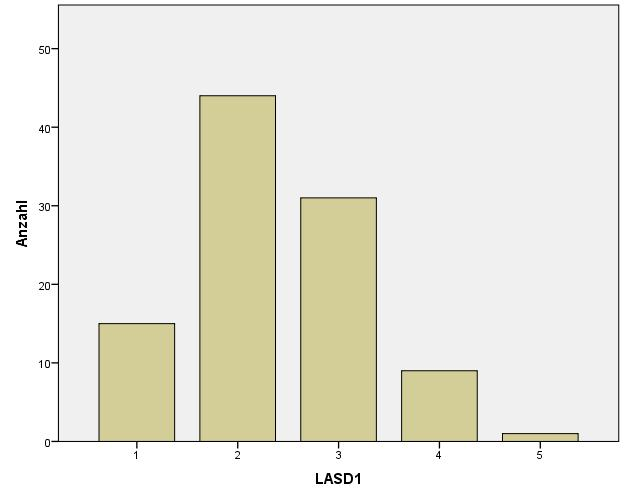
\includegraphics{pics/SPSS_LASD1_hist.jpg}
\caption{Histogramm LASD1 in SPSS}
\end{figure}

\hypertarget{bildung-des-mittelwerts-spss-syntax}{%
\subsection{Bildung des Mittelwerts (SPSS Syntax)}\label{bildung-des-mittelwerts-spss-syntax}}

COMPUTE SD=MEAN(LASD1, LASD2, LASD3, LASD4, LASD5, LASD6, LASD7, LASD8, LASD9, LASD10).
EXECUTE.

Alternativer Syntax:

\begin{itemize}
\tightlist
\item
  Daten sortieren
\item
  MEAN(LASD1 to LASD10)
\end{itemize}

\begin{figure}
\centering
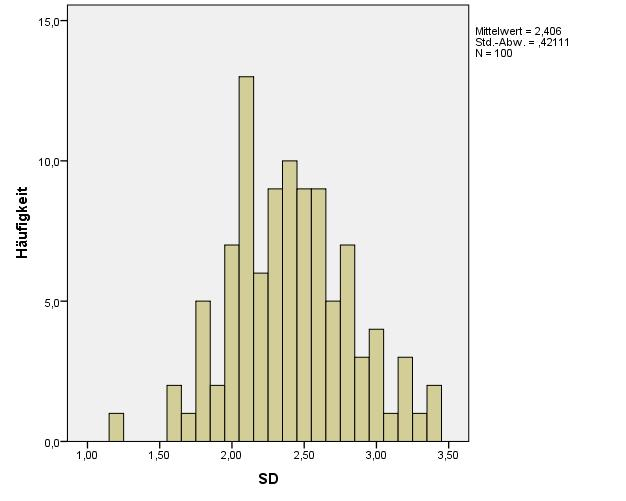
\includegraphics{pics/SPSS_SD_hist.jpg}
\caption{Histogramm SD in SPSS}
\end{figure}

\hypertarget{inferenzstatistik-schlieuxdfende-statistik}{%
\chapter{Inferenzstatistik (schließende Statistik)}\label{inferenzstatistik-schlieuxdfende-statistik}}

Video: \url{https://youtu.be/-63gq7Q1rBM}

\hypertarget{anknuxfcpfungspunkte-2}{%
\section{Anknüpfungspunkte}\label{anknuxfcpfungspunkte-2}}

\begin{itemize}
\tightlist
\item
  Signifikanztest
\item
  Lagemaße
\item
  Streuungsmaße
\item
  z-Transformation
\end{itemize}

\hypertarget{vorbereitung-2}{%
\section{Vorbereitung}\label{vorbereitung-2}}

\hypertarget{allgemeines-2}{%
\section{Allgemeines}\label{allgemeines-2}}

\begin{itemize}
\tightlist
\item
  Ziel: Schluss von den erhobenen Daten einer Stichprobe auf die Werte in der Population
\end{itemize}

\hypertarget{schuxe4tzer}{%
\subsection{Schätzer}\label{schuxe4tzer}}

\begin{itemize}
\tightlist
\item
  Punktschätzung: Angabe eines Werts für einen unbekannten Parameter

  \begin{itemize}
  \tightlist
  \item
    Erwartungswert \(E(X)\)
  \item
    Probleme: (fast) sicher falsch, keine Aussage über Genauigkeit
  \end{itemize}
\item
  Intervallschätzung: Angabe eines Intervalls, das mit einer bestimmten Wahrscheinlichkeit den unbekannten Parameter überdeckt.

  \begin{itemize}
  \tightlist
  \item
    Konfidenzintervall (confidence interval, CI): Der Wertebereich, in dem man den interessierenden Parameter
    der Grundgesamtheit mit einer bestimmten Wahrscheinlichkeit erwartet,
    bezeichnet man als Konfidenzintervall.
  \end{itemize}
\item
  Hypothesentest: Annahme bzw. Zurückweisung von Aussagen über den unbekannten Parameter bei einer vorgegeben Irrtumswahrscheinlichkeit
\end{itemize}

\hypertarget{standardfehler-se-des-mittelwerts}{%
\section{Standardfehler (SE) des Mittelwerts}\label{standardfehler-se-des-mittelwerts}}

\begin{itemize}
\tightlist
\item
  Genauigkeit der Schätzung: Der Standardfehler des Mittelwerts gibt die Genauigkeit der Schätzung des Populationsmittelwerts an. Aufgrund einer Stichprobe können wir nicht nur den Mittelwert der Population schätzen, sondern auch die Genauigkeit dieser Schätzung bestimmen.
\item
  Streuung in einer Verteilung: Der Standardfehler ist definiert als die Streuung in einer Verteilung von Mittelwerten aus gleich großen Zufallsstichproben einer Population.
\item
  Je kleiner der Standardfehler, desto präziser die Schätzung des Populationsparameters
\item
  Standardfehler wird größer\ldots{}

  \begin{itemize}
  \tightlist
  \item
    je größer die Streuung der Messwerte \(\sigma\)
  \item
    je kleiner die Stichprobe \(n\)
  \end{itemize}
\end{itemize}

\[ SE = \frac{\sigma}{\sqrt{n}} \approx \frac{s}{\sqrt{n}}\]

\hypertarget{konfidenzintervall-ci}{%
\section{Konfidenzintervall (CI)}\label{konfidenzintervall-ci}}

\begin{itemize}
\tightlist
\item
  Der Konfidenzintervall ergibt sich aus

  \begin{itemize}
  \tightlist
  \item
    der gesetzten Breite des Intervalls \(z\) (\(\alpha\)-Level)
    - Per Konvention: z = 1,96 (95\%) oder 2,58 (99\%), siehe z-Transformation
  \item
    dem Stichprobenmittelwert \(\bar{x}\)
  \item
    dem geschätzen Standardfehler \(SE_{\bar{x}}\)
    \[ lower limit (LL) = \bar{x} - z * SE_{\bar{x}} \]
    \[ upper limit (UL) = \bar{x} + z * SE_{\bar{x}} \]
  \end{itemize}
\item
  Interpretation: Misst man mehrmals und berechnet jeweils den 95\% CI, enthalten 95\% der Intervalle den Populations-Mittelwert.

  \begin{itemize}
  \tightlist
  \item
    falsche Interpretation: ``Mit einer Wahrscheinlichkeit von 95\% liegt der Populations-Mittelwert innerhalb von dem CI''
  \end{itemize}
\end{itemize}

\hypertarget{konfidenzintervall-ci---berechnungsbeispiel-in-r}{%
\section{Konfidenzintervall (CI) - Berechnungsbeispiel in R}\label{konfidenzintervall-ci---berechnungsbeispiel-in-r}}

\begin{Shaded}
\begin{Highlighting}[]
\NormalTok{data <-}\StringTok{ }\KeywordTok{c}\NormalTok{(}\DecValTok{1}\NormalTok{, }\DecValTok{2}\NormalTok{, }\DecValTok{10}\NormalTok{, }\DecValTok{5}\NormalTok{, }\DecValTok{20}\NormalTok{, }\DecValTok{3}\NormalTok{)}
\NormalTok{m <-}\StringTok{ }\KeywordTok{mean}\NormalTok{(data)}
\NormalTok{sd <-}\StringTok{ }\KeywordTok{sd}\NormalTok{(data)}
\NormalTok{n <-}\StringTok{ }\KeywordTok{length}\NormalTok{(data)}
\NormalTok{SE <-}\StringTok{ }\NormalTok{sd}\OperatorTok{/}\KeywordTok{sqrt}\NormalTok{(n)}
\NormalTok{(LL <-}\StringTok{ }\NormalTok{m }\OperatorTok{-}\StringTok{ }\FloatTok{1.96}\OperatorTok{*}\NormalTok{SE)}
\end{Highlighting}
\end{Shaded}

\begin{verbatim}
## [1] 1.1
\end{verbatim}

\begin{Shaded}
\begin{Highlighting}[]
\NormalTok{(UL <-}\StringTok{ }\NormalTok{m }\OperatorTok{+}\StringTok{ }\FloatTok{1.96}\OperatorTok{*}\NormalTok{SE)}
\end{Highlighting}
\end{Shaded}

\begin{verbatim}
## [1] 13
\end{verbatim}

Der 95\% Konfidenzintervall um den Mittelwert 6.83 reicht von 1.08 bis 12.59.

\hypertarget{konfidenzintervall-ci---weite}{%
\section{Konfidenzintervall (CI) - Weite}\label{konfidenzintervall-ci---weite}}

\begin{itemize}
\tightlist
\item
  Die Länge des Konfidenzintervalls (UL-LL) hängt ab von

  \begin{itemize}
  \tightlist
  \item
    \(\alpha\)-Level / z: Je größer das Alpha-Level, desto weiter das CI
  \item
    \(\sigma\): Je größer die Standardabweichung, desto weiter das CI
  \item
    n: Je größer die Stichprobe, desto kürzer das CI
  \end{itemize}
\end{itemize}

\[ UL - LL = \bar{x} + \alpha*SE -(\bar{x} - \alpha*SE) = 2*\alpha*SE = \frac{2*\alpha*\sigma}{\sqrt{n}} \]

\begin{itemize}
\tightlist
\item
  Interpretation: ein weites CI ist ``ungenauer''!
\end{itemize}

Video: \url{https://youtu.be/agjKK6_bSrA}

\hypertarget{demonstration-von-population-stichprobenziehung-standardfehler}{%
\section{Demonstration von Population, Stichprobenziehung, Standardfehler}\label{demonstration-von-population-stichprobenziehung-standardfehler}}

\hypertarget{population}{%
\subsection{Population}\label{population}}

Wir generieren eine Punktwolke, die für diese Demonstration unsere Grundgesamtheit darstellt. Es sind 100 Datenpunkte mit 2 Variablen x und y. Die Regressionsgleichung der Population ist:

\[ y = 1 + 2x + e \]

Hier ist die Punktewolke dargestellt:

\includegraphics{reflektion_files/figure-latex/unnamed-chunk-34-1.pdf}

\hypertarget{stichprobe}{%
\subsection{Stichprobe}\label{stichprobe}}

Wir ziehen nun 4 Stichproben (ca. 0.1 der Population werden jeweils gesampelt) von dieser Grundgesamtheit (rote Punkte) und zeichnen die Regressionsgerade ein (rote Linie). Die Stichproben sind immer anders, und daraus ergibt sich auch ein andere Regressionslinie. Der Konfidenzintervall (grauer Bereich) verändert sich ebenfalls um die Regressionslinie herum -- je nachdem wie, die Stichprobe gestreut ist.

\includegraphics{reflektion_files/figure-latex/unnamed-chunk-36-1.pdf}

Im Histogramm werden die B-Werte aller Stichproben gesammelt.

\includegraphics{reflektion_files/figure-latex/unnamed-chunk-37-1.pdf}

\hypertarget{gruxf6uxdfere-stichprobe}{%
\subsection{Größere Stichprobe}\label{gruxf6uxdfere-stichprobe}}

Jetzt wiederholen wir den Versuch mit eine größeren Stichprobe (ca. 0.6 der Population werden jeweils gesampelt).

\begin{quote}
\textbf{Frage:} Wie verändern sich die Standardfehler?
\end{quote}

\includegraphics{reflektion_files/figure-latex/unnamed-chunk-39-1.pdf}

\includegraphics{reflektion_files/figure-latex/unnamed-chunk-41-1.pdf}

\hypertarget{uxfcbung}{%
\section{Übung}\label{uxfcbung}}

\begin{enumerate}
\def\labelenumi{\arabic{enumi}.}
\tightlist
\item
  Lade die Daten Froehlich et al.~2014 Daten 100.sav
\item
  Berechne eine neue Variable: MWC = der Mittelwert von WC1-WC7. Welchen Wert hat Fall 3?
\item
  Welches Messniveau hat MWC?
\item
  Berechne den Standardfehler mit der Hand und kontrolliere den Wert in SPSS.
\item
  Erstelle ein Diagramm, das MWC in Balken (inkl. 99\% Konfidenzintervall) für die einzelnen Banken (DBAN) zeigt. Welche Bank hat den höchsten MWC Wert (ohne Fehler)?
\end{enumerate}

\hypertarget{luxf6sung-1}{%
\section{Lösung}\label{luxf6sung-1}}

\begin{enumerate}
\def\labelenumi{\arabic{enumi}.}
\item
  \begin{itemize}
  \item
  \end{itemize}
\item
  Transformieren, Variable Berechnen, MEAN(WC1, WC2,.). 3,85714285714286
\item
  Metrisch.
\item
  SPSS: via Häufigkeiten, Mit der Hand: Standardabweichung / Wurzel(n). SE = ,05948
\item
  Bank 3
\end{enumerate}

\hypertarget{hypothesentests}{%
\chapter{Hypothesentests}\label{hypothesentests}}

\hypertarget{anknuxfcpfungspunkte-3}{%
\section{Anknüpfungspunkte}\label{anknuxfcpfungspunkte-3}}

\begin{itemize}
\tightlist
\item
  Konfidenzintervalle
\end{itemize}

\hypertarget{vorbereitung-3}{%
\section{Vorbereitung}\label{vorbereitung-3}}

\begin{itemize}
\tightlist
\item
  OS3: 4
\item
  IS: 9
\item
  Ps: 13
\item
  K13: 6
\item
  Video: \url{https://www.khanacademy.org/math/statistics-probability/confidence-intervals-one-sample}
\item
  Video: \url{https://www.khanacademy.org/math/statistics-probability/significance-tests-one-sample\#idea-of-significance-tests}
\end{itemize}

\hypertarget{problemstellung-1}{%
\section{Problemstellung}\label{problemstellung-1}}

Wir möchten feststellen, ob sich basierend auf unserer Stichprobe ein Unterschied oder ein Zusammenhang von Variablen in der Grundgesamtheit feststellen lässt.

\hypertarget{allgemeines-3}{%
\section{Allgemeines}\label{allgemeines-3}}

\begin{itemize}
\tightlist
\item
  Ziel: Hypothesen über die unbekannte Grundgesamtheit anhand einer Stichprobe testen
\item
  Forschungshypothese/Alternativhypothese (H1): sagt häufig aus, dass ein Effekt präsent ist bzw. Unterschiede existieren oder ein Zusammenhang besteht.
\item
  Nullhypothese (H0): sagt häufig aus, dass kein Effekt bzw. Unterschied vorliegt oder dass ein bestimmter Zusammenhang nicht besteht.
\end{itemize}

\hypertarget{beispiel}{%
\subsection{Beispiel}\label{beispiel}}

\begin{itemize}
\tightlist
\item
  H1: Männer und Frauen verdienen in Österreich im Durchschnitt unterschiedlich viel.
\item
  H0: Männer und Frauen verdienen in Österreich im Durchschnitt gleich viel.

  \begin{itemize}
  \tightlist
  \item
    noch klarer: Männer und Frauen verdienen in Österreich im Durchschnitt \emph{nicht unterschiedlich} viel.
  \end{itemize}
\end{itemize}

\hypertarget{logik-der-nullhypothese}{%
\section{Logik der Nullhypothese}\label{logik-der-nullhypothese}}

\begin{itemize}
\tightlist
\item
  Wir gehen davon aus, dass die Nullhypothese zutrifft und schauen unser Stichprobenergebnis an. Ist dieses sehr unwahrscheinlich unter Gültigkeit der Nullhypothese, so weisen wir die Nullhypothese zurück und akzeptieren die Alternativhypothese.
\item
  Aber: weder Nullhypothese noch Alternativhypothese können auf der Basis eines Signifikanztests ``bewiesen'' werden!
\end{itemize}

\hypertarget{signifikanztest}{%
\section{Signifikanztest}\label{signifikanztest}}

Ein statistischer Test (Signifikanztest) ist ein Verfahren, das es erlaubt auf der Basis einer Stichprobe mit einer gewissen Irrtumswahrscheinlichkeit zwischen zwei konkurrierenden wissenschaftlichen Hypothesen zu entscheiden.

Wenn es eine hinreichende Übereinstimmung zwischen der Hypothese und der Beobachtung gibt, ist die Hypothese vorläufig unterstützt.

\hypertarget{exkurs-geschichte}{%
\section{Exkurs: Geschichte}\label{exkurs-geschichte}}

\begin{itemize}
\tightlist
\item
  John Arbuthnot (1667-1735): Leibarzt von Queen Anne
\item
  Auszählung von Geburtsregistern von 82 Jahrgängen
\item
  Anzahl der Knabengeburten (K = 82) \textgreater{} Anzahl der Mädchengeburten (M = 0)
\item
  Wie wahrscheinlich ist das (bei Gültigkeit der Nullhypothese)?
\end{itemize}

\[ H0: P(K) = P(M) = 0.5 \]

\hypertarget{wahrscheinlichkeit}{%
\section{Wahrscheinlichkeit}\label{wahrscheinlichkeit}}

\begin{itemize}
\tightlist
\item
  Verteilung bekannt: Die Teststatistik hat bekannte Eigenschaften: wir wissen, wie häufig bestimmte Werte dieser Verteilung auftreten (z.B. auf der Basis der Normalverteilung)
\item
  Wahrscheinlichkeit berechenbar: wir können berechnen, wie wahrscheinlich es ist dieses Stichprobenergebnis oder ein noch extremeres zu erhalten, vorausgesetzt, dass kein Effekt/Zusammenhang in der Grundgesamtheit besteht.
\item
  \(p\)-Wert
\end{itemize}

\hypertarget{schritte-eines-hypothesentests}{%
\section{Schritte eines Hypothesentests}\label{schritte-eines-hypothesentests}}

\begin{itemize}
\tightlist
\item
  Test wählen
\item
  Voraussetzungen prüfen

  \begin{itemize}
  \tightlist
  \item
    Skalenniveau der Daten
  \item
    Randomisierung
  \item
    Verteilung der Variablen
  \item
    Stichprobengröße
  \end{itemize}
\item
  Hypothesen aufstellen

  \begin{itemize}
  \tightlist
  \item
    Nullhypothese
  \item
    Alternativhypothese
  \end{itemize}
\item
  Teststatistik berechnen
\item
  \(p\)-Wert berechnen
\item
  Schlussfolgerung

  \begin{itemize}
  \tightlist
  \item
    Ablehnung der H0 und Annahme der H1 oder Beibehaltung der H0.
  \end{itemize}
\end{itemize}

\hypertarget{fehler-im-hypothesentest}{%
\section{Fehler im Hypothesentest}\label{fehler-im-hypothesentest}}

\begin{itemize}
\tightlist
\item
  \(\alpha\)-Fehler = Fehler 1. Art; \(p = \alpha\) : H0 ist wahr, H0 wird aber verworfen. Entscheidung für die Alternativhypothese, obwohl die Nullhypothese richtig ist.
\item
  \(\beta\)-Fehler = Fehler 2. Art: H1 ist wahr, H0 wird aber nicht verworfen. Entscheidung für die Nullhypothese, obwohl die Alternativhypothese richtig ist.
\item
  Die Fehler sind abhängig voneinander: Verringert man den Fehler 1. Art, so erhöht man gleichzeitig den Fehler 2. Art.
\end{itemize}

\begin{longtable}[]{@{}lll@{}}
\toprule
~ & H0 wahr & H0 falsch\tabularnewline
\midrule
\endhead
H0 annehmen & OK & \(\beta\)\tabularnewline
H0 ablehnen & \(\alpha\) & OK\tabularnewline
\bottomrule
\end{longtable}

\hypertarget{faq}{%
\section{FAQ}\label{faq}}

\textbf{Frage:} Bei einer Regression von Ablenkbarkeit auf Zeitmanagement ist p = 0.029. Was bedeutet das?

\textbf{Antwort:} Es gibt eine Wahrscheinlichkeit (p) von 2,9\% aufgrund der Stichprobe zu sagen, dass Zeitmanagement einen Einfluss auf Ablenkbarkeit hat, obwohl es diesen Effekt in der Grundgesamtheit nicht gibt".

\hypertarget{uxfcbungen-2}{%
\section{Übungen}\label{uxfcbungen-2}}

\hypertarget{bilde-je-eine-hypothese}{%
\subsection{(1) Bilde je eine Hypothese:}\label{bilde-je-eine-hypothese}}

\begin{itemize}
\tightlist
\item
  mit Lehrerzufriedenheit als unabhängige Variable und Schulklima als abhängige Variable. - mit Schulklima als unabhängige Variable und Lehrerzufriedenheit als abhängige Variable.
\item
  mit Lehrerzufriedenheit und Schulklima als unabhängigen Variablen.
\end{itemize}

\hypertarget{was-ist-an-den-folgenden-hypothesen-gutschlecht}{%
\subsection{(2) Was ist an den folgenden Hypothesen gut/schlecht:}\label{was-ist-an-den-folgenden-hypothesen-gutschlecht}}

\begin{itemize}
\item
  \begin{enumerate}
  \def\labelenumi{(\alph{enumi})}
  \tightlist
  \item
    Unter welchen Bedingungen lassen sich Lernstrategien auf neue Situationen übertragen? - (b) Junge Lehrer sind bei den Schülern beliebter, weil sie die Interessen der Schüler besser kennen.
  \end{enumerate}
\item
  \begin{enumerate}
  \def\labelenumi{(\alph{enumi})}
  \setcounter{enumi}{2}
  \tightlist
  \item
    Burschen aus höheren sozialen Schichten werden von männlichen Lehrkräften im Mathematikunterricht stärker gefördert.
  \end{enumerate}
\item
  \begin{enumerate}
  \def\labelenumi{(\alph{enumi})}
  \setcounter{enumi}{3}
  \tightlist
  \item
    Antiautoritäre Erziehung macht frei.
  \end{enumerate}
\item
  \begin{enumerate}
  \def\labelenumi{(\alph{enumi})}
  \setcounter{enumi}{4}
  \tightlist
  \item
    Lehrer sind nicht bereit, auf alternative Formen der Leistungsbeurteilung umzusteigen, unter dem Vorwand, dass die Eltern großen Wert auf Ziffernnoten
    legen.
  \end{enumerate}
\item
  \begin{enumerate}
  \def\labelenumi{(\alph{enumi})}
  \setcounter{enumi}{5}
  \tightlist
  \item
    Prüfungsangst vermindert die Punktzahl bei einem Leistungstest.
  \end{enumerate}
\item
  \begin{enumerate}
  \def\labelenumi{(\alph{enumi})}
  \setcounter{enumi}{6}
  \tightlist
  \item
    Schüler werden auf Grund ihrer sozialen Herkunft in die Sonderschule abgeschoben.
  \end{enumerate}
\item
  \begin{enumerate}
  \def\labelenumi{(\alph{enumi})}
  \setcounter{enumi}{7}
  \tightlist
  \item
    Junge Lehrer sind engagierter.
  \end{enumerate}
\item
  \begin{enumerate}
  \def\labelenumi{(\roman{enumi})}
  \tightlist
  \item
    Autoritäres Lehrerverhalten führt zu einem schlechten Lernerfolg.
  \end{enumerate}
\item
  \begin{enumerate}
  \def\labelenumi{\alph{enumi})}
  \setcounter{enumi}{9}
  \tightlist
  \item
    Das Verhalten bei Fingermalaufgaben wird von der sozialen Schichtzugehörigkeit beeinflusst.
  \end{enumerate}
\item
  \begin{enumerate}
  \def\labelenumi{(\alph{enumi})}
  \setcounter{enumi}{10}
  \tightlist
  \item
    Gruppenarbeit ist gut für Kinder.
  \end{enumerate}
\item
  \begin{enumerate}
  \def\labelenumi{(\alph{enumi})}
  \setcounter{enumi}{11}
  \tightlist
  \item
    Ziffernnoten sind bei Lehrern beliebter, weil sie weniger Arbeit machen.
  \end{enumerate}
\item
  \begin{enumerate}
  \def\labelenumi{(\alph{enumi})}
  \setcounter{enumi}{12}
  \tightlist
  \item
    Hat Angst Auswirkungen auf die Leistung?
  \end{enumerate}
\end{itemize}

\hypertarget{formulieren-sie-hypothesen-zu-folgenden-themen}{%
\subsection{(3) Formulieren Sie Hypothesen zu folgenden Themen:}\label{formulieren-sie-hypothesen-zu-folgenden-themen}}

\begin{itemize}
\item
  \begin{enumerate}
  \def\labelenumi{(\alph{enumi})}
  \tightlist
  \item
    Essstörungen bei Mädchen und Buben in verschiedenen Schultypen
  \end{enumerate}
\item
  \begin{enumerate}
  \def\labelenumi{(\alph{enumi})}
  \setcounter{enumi}{1}
  \tightlist
  \item
    Vergleich der Schulnoten zwischen 2. und 7. Klasse AHS
  \end{enumerate}
\item
  \begin{enumerate}
  \def\labelenumi{(\alph{enumi})}
  \setcounter{enumi}{2}
  \tightlist
  \item
    Berufszufriedenheit von Lehrern
  \end{enumerate}
\item
  \begin{enumerate}
  \def\labelenumi{(\alph{enumi})}
  \setcounter{enumi}{3}
  \tightlist
  \item
    Vergleich der Englischkenntnisse zwischen österreichischen und Migrantenkindern
  \end{enumerate}
\end{itemize}

\hypertarget{luxf6sungen}{%
\section{Lösungen}\label{luxf6sungen}}

\hypertarget{luxf6sung-2}{%
\subsection{(1) Lösung}\label{luxf6sung-2}}

\begin{itemize}
\tightlist
\item
  Die Lehrerzufriedenheit hat einen Einfluss auf das Schulklima.
\item
  Das Schulklima wirkt sich auf die Lehrerzufriedenheit aus.
\item
  Die Lehrerzufriedenheit und das Schulklima beeinflussen die Noten der Schüler.
\end{itemize}

\hypertarget{luxf6sung-3}{%
\subsection{(2) Lösung}\label{luxf6sung-3}}

\begin{itemize}
\tightlist
\item
  Das ist keine Hypothese sondern eine Frage. Eine Hypothese wäre eine (vermutete) Antwort auf diese Frage.
\item
  Es ist (fast) unmöglich, durch quantitative Forschung festzustellen, warum etwas so
  ist. Besser wäre daher, den zweiten Teil der Hypothese zu streichen.
\item
  \ldots als wer? Als Burschen aus niedrigen sozialen Schichten? Als Mädchen aus höheren sozialen Schichten? Als Burschen von weiblichen Lehrkräften? Als Mädchen im Englischunterricht? Antwort: Zu viele Fragestellungen in eine Hypothese gepackt. Ausformuliert wären das 3-4 Hypothesen.
\item
  Macht wen frei? ``Freiheit'' ist schwer zu messen. Und selbst wenn, kann man nur schwer feststellen, ob antiautoritäre Erziehung tatsächlich der Grund dafür ist.
\item
  Es ist durch quantitative Forschung sehr schwer festzustellen, ob der Elternwunsch
  von den Lehrern als Vorwand benutzt wird, oder ob er der tatsächliche Grund ist. Jedenfalls müssten dazu Lehrer und Eltern befragt werden.
\item
  Gut.
\item
  Es ist durch quantitative Forschung sehr schwer festzustellen, ob Schüler auf Grund
  ihrer sozialen Herkunft abgeschoben werden. Die Feststellung, dass Schüler aus unteren sozialen Schichten in der Sonderschule überrepräsentiert sind, würde diese Hypothese jedenfalls nicht bestätigen. Es ist nämlich genauso gut möglich, dass Schüler aus unteren sozialen Schichten zu Hause weniger gefördert werden, daher schlechtere Schulleistungen erbringen, und daher auf Grund der Schulleistungen in die Sonderschule überstellt werden. - \ldots als wer? ``Engagiertheit'' ist sehr schwer quantitativ zu erfassen. Wann ist jemand engagiert?
\item
  \ldots bei wem? ``Autorität'' ist sehr schwer quantitativ zu erfassen. Wann ist jemand autoritär?
\item
  ``Verhalten'' ist zu allgemein. Welches Verhalten?
\item
  Was heißt ``gut''?
\item
  Warum Ziffernnoten beliebter sind, ist durch quantitative Forschung sehr schwer herauszufinden. Es muss damit gerechnet werden, dass Lehrer sozial erwünscht antworten und andere Gründe vorgeben.
\item
  Das ist keine Hypothese sondern eine Frage. Auswirkung auf welche Leistung?
\end{itemize}

\hypertarget{luxf6sungen-1}{%
\subsection{(3) Lösungen}\label{luxf6sungen-1}}

\begin{itemize}
\tightlist
\item
  Essstörungen treten sowohl in der AHS als auch in der BHS bei Mädchen häufiger auf als bei Buben.
\item
  Die Streuung der Geschichtenoten ist in der 7. Klasse geringer als in der 2. Klasse.
\item
  Die Berufszufriedenheit von Lehrern nimmt mit dem Dienstalter ab.
\item
  In der 2. Klasse AHS unterscheiden sich die Englischnoten österreichischer Kinder nicht von den Englischnoten von Migrantenkindern.
\end{itemize}

\hypertarget{visualisierung}{%
\chapter{Visualisierung}\label{visualisierung}}

\hypertarget{allgemeines-4}{%
\section{Allgemeines}\label{allgemeines-4}}

Jede Darstellung sollte selbsterklärend sein -- daher ist auf aussagekräftige Titel, Achsenbeschriftungen und Legenden zu achten! Generell sollte auf Lesbarkeit optimiert werden und die Kernaussage bzw. das Ziel der Darstellung klar erkennbar sein (und eventuell im Titel direkt benannt werden). {[}Achtung, das passiert auf Grund von Platzlimitationen in diesem Skriptum nicht immer!{]}

\hypertarget{histogramm}{%
\section{Histogramm}\label{histogramm}}

Ein Histogramm gibt die Häufigkeitsverteilung einer Variablen wieder. Dafür werden die Daten in Klassen (bins) eingeteilt--die Festsetzung der bins verändert die Darstellung teilweise enorm.

\includegraphics{reflektion_files/figure-latex/unnamed-chunk-43-1.pdf}

\hypertarget{boxplot}{%
\section{Boxplot}\label{boxplot}}

Ein Boxplot ist eine kompakte Darstellung der Quartile einer Variable durch eine \emph{Box} und \emph{Whisker} (daher wird diese Darstellung auch Box-and-Whisker-Plot genannt). Es gibt verschiedene Varianten, die folgende verwendet folgende Definitionen:

\begin{itemize}
\tightlist
\item
  Die Striche gehen von \(Q1 - 1.5*IQR\) bis \(Q3 + 1.5*IQR\).
\item
  Die Punkte sind ``Ausreißer'' (außerhalb der von den Strichen erfassten Daten)s
\item
  Die Boxen definieren Q1 bzw. Q3
\item
  Der Median (Q2) ist der (horizontale) Balken innerhalb der Box
\end{itemize}

\includegraphics{reflektion_files/figure-latex/unnamed-chunk-44-1.pdf}

\hypertarget{scatterplot}{%
\section{Scatterplot}\label{scatterplot}}

Der Scatterplot stellt eine Punktwolke basierend auf 2 kontinuierlichen Variablen dar.

\includegraphics{reflektion_files/figure-latex/unnamed-chunk-45-1.pdf}

Die Regressionsgerade kann zusätzlich eingezeichnet werden.

\includegraphics{reflektion_files/figure-latex/unnamed-chunk-46-1.pdf}

Der Konfidenzintervall kann zusätzlich eingezeichnet werden.

\includegraphics{reflektion_files/figure-latex/unnamed-chunk-47-1.pdf}

\hypertarget{bar-chart}{%
\section{Bar-Chart}\label{bar-chart}}

\includegraphics{reflektion_files/figure-latex/unnamed-chunk-48-1.pdf}

Es sollten keine Verzerrungen der Proportionen entstehen:

\includegraphics{reflektion_files/figure-latex/unnamed-chunk-49-1.pdf}

\hypertarget{t-test-und-u-test}{%
\chapter{t-test und U-Test}\label{t-test-und-u-test}}

\hypertarget{problemstellung-2}{%
\section{Problemstellung}\label{problemstellung-2}}

Wir möchten herausfinden, ob es einen Unterschied bei der Einschätzung der \emph{Lernkultur} basierend auf dem \emph{Geschlecht} der StudienteilnehmerInnen gibt.

\hypertarget{anknuxfcpfungspunkte-4}{%
\section{Anknüpfungspunkte}\label{anknuxfcpfungspunkte-4}}

\begin{itemize}
\tightlist
\item
  Unterschiedshypothese
\item
  Hypothesentest
\end{itemize}

\hypertarget{allgemeines-5}{%
\section{Allgemeines}\label{allgemeines-5}}

\begin{itemize}
\tightlist
\item
  Ziel: Vergleich von zwei Stichprobenmittelwerten
\item
  Arten

  \begin{itemize}
  \tightlist
  \item
    unabhängige Stichproben: Keine Beobachtung bzw. Messung wird von einer anderen beeinflusst. Beispiel: eine Gruppe StudentInnen wird zufällig in zwei gleichgroÃ\textless U+009F\textgreater e Gruppen geteilt. Gruppe 1 nimmt an einem Lerntutorium teil, Gruppe 2 nicht. Die zwei Gruppen sind unabhängig voneinander.
  \item
    abhängige Stichproben: die Messungen werden voneinander beeinflusst. Beispiel: eine Gruppe von StudentInnen nimmt an einem Lerntutorium teil. Ein Forscher vergleicht sodann die Lernkompetenz der StudentInnen vor und nach dem Lerntutorium.
  \end{itemize}
\item
  Hypothesentest

  \begin{itemize}
  \tightlist
  \item
    H0: es existiert kein Unterschied zwischen zwei Gruppen.
  \item
    H1: es existiert ein Unterschied zwischen zwei Gruppen.
  \end{itemize}
\item
  Logik des t-Tests

  \begin{itemize}
  \tightlist
  \item
    Gruppenmittelwerte berechnen
  \item
    Differenz der Gruppenmittelwerte berechnen
  \item
    Signifikanz der Differenz berechnen
  \end{itemize}
\end{itemize}

\hypertarget{voraussetzungen-t-test}{%
\section{Voraussetzungen t-Test}\label{voraussetzungen-t-test}}

\begin{itemize}
\tightlist
\item
  Randomisierung = Zufallsstichprobe
\item
  mindestens intervallskalierte Daten. Bei ordinalskalierten Daten kannst du auf den Mann-Whitney-U-Test (unabhängige Stichproben) bzw. den Wilcoxon-Vorzeichen-Rang-Test (gepaarte Stichproben) ausweichen.
\item
  Normalverteilung der Variablen. Test: Kolmogorov-Smirnov-Test (sollte nicht signifikant sein!). Bei nicht normalverteilten Daten kannst du auf den Mann-Whitney-U-Test (unabhängige Stichproben) bzw. den Wilcoxon-Vorzeichen-Rang-Test (gepaarte Stichproben) ausweichen.
\item
  Varianzhomogenität: gleiche Varianzen der Gruppen. Test: Levene-Test (Ergibt sich hier ein signifikanter F-Wert, dann darf nicht von Varianzhomogenität ausgegangen werden)
\end{itemize}

\hypertarget{beispiel-1}{%
\section{Beispiel}\label{beispiel-1}}

Datei: ttest1.csv (Simulierte Daten)

\begin{itemize}
\tightlist
\item
  Variablen

  \begin{itemize}
  \tightlist
  \item
    Wert
  \item
    Gruppe (0, 1, 2)

    \begin{itemize}
    \tightlist
    \item
      0 bzw. 1 = zufällig Daten (``männlich / weiblich'')
    \item
      2 = manipulierte Daten
    \end{itemize}
  \end{itemize}
\end{itemize}

\hypertarget{umsetzung-mit-software}{%
\section{Umsetzung mit Software}\label{umsetzung-mit-software}}

In SPSS:

Video: \url{https://youtu.be/yCa3fryPOa4}

In PSPP:

Video: \url{https://youtu.be/orqwKyuc1y0}

\hypertarget{beispiel---visualisierung}{%
\subsection{Beispiel - Visualisierung}\label{beispiel---visualisierung}}

Diese drei \textbf{Boxplots} zeigen die Verteilungen von ``Wert'' in den drei Gruppen (0, 1, 2).

\includegraphics{reflektion_files/figure-latex/unnamed-chunk-50-1.pdf}

\hypertarget{beispiel---t-test-gruppen-01}{%
\subsection{Beispiel - t-Test Gruppen 0/1}\label{beispiel---t-test-gruppen-01}}

Wir führen einen t-Test zwischen den Gruppen 0 und 1 durch.

\begin{verbatim}
## 
##  Welch Two Sample t-test
## 
## data:  df$Wert[df$Gruppe == 0] and df$Wert[df$Gruppe == 1]
## t = 0.5, df = 100, p-value = 0.6
## alternative hypothesis: true difference in means is not equal to 0
## 95 percent confidence interval:
##  -0.26  0.42
## sample estimates:
## mean of x mean of y 
##     0.043    -0.036
\end{verbatim}

\hypertarget{beispiel---t-test-gruppen-01-interpretation}{%
\subsection{Beispiel - t-Test Gruppen 0/1: Interpretation}\label{beispiel---t-test-gruppen-01-interpretation}}

Beachte bei der Interpretation\ldots{}

\begin{itemize}
\tightlist
\item
  den Konfidenzintervall von -0.26 bis 0.42
\item
  den p-Wert von 0.65
\end{itemize}

\begin{quote}
\textbf{Frage:} Was sagen diese Werte aus?
\end{quote}

\hypertarget{beispiel---t-test-gruppen-02}{%
\subsection{Beispiel - t-Test Gruppen 0/2}\label{beispiel---t-test-gruppen-02}}

Wir führen einen t-Test zwischen den Gruppen 0 und 2 durch.

\begin{verbatim}
## 
##  Welch Two Sample t-test
## 
## data:  df$Wert[df$Gruppe == 0] and df$Wert[df$Gruppe == 2]
## t = -6, df = 100, p-value = 2e-08
## alternative hypothesis: true difference in means is not equal to 0
## 95 percent confidence interval:
##  -1.32 -0.66
## sample estimates:
## mean of x mean of y 
##     0.043     1.029
\end{verbatim}

\hypertarget{beispiel---t-test-gruppen-02-interpretation}{%
\subsection{Beispiel - t-Test Gruppen 0/2: Interpretation}\label{beispiel---t-test-gruppen-02-interpretation}}

Beachte bei der Interpretation\ldots{}

\begin{itemize}
\tightlist
\item
  den Konfidenzintervall von -1.32 bis -0.66
\item
  den p-Wert von 0
\end{itemize}

\begin{quote}
\textbf{Achtung:} Der p-Wert ist natürlich nicht genau 0 (siehe Output des Tests)--aber durch Rundungen könnte es so aussehen. Bei eigenen Texten bzw. der Interpretation daher \emph{\textless{} 0.001} verwenden.
\end{quote}

und, da es sich um ein \textbf{statistisch signifikantes Ergebnis} handelt

\begin{itemize}
\tightlist
\item
  die Mittelwerte der Gruppen von 0.04 bzw. 1.03.
\end{itemize}

\begin{quote}
\textbf{Frage:} Was sagen diese Werte aus?
\end{quote}

\hypertarget{uxe3bung}{%
\section{Übung}\label{uxe3bung}}

\begin{enumerate}
\def\labelenumi{\arabic{enumi}.}
\item
  Lade die Daten Froehlich 2014 Daten 100.sav
\item
  Führe den Kolmogorov-Smirnov (K-S) Test für die Variablen WC1 bis WC7 durch. Was wird hier getestet?
\item
  Was bedeuten signifikante Ergebnisse im K-S Test?
\item
  Wie lautet H0 des K-S Test?
\item
  Wie viele der getesteten Variablen WC1 bis WC7 sind laut K-S Test wahrscheinlich normalverteilt?
\item
  Führe den Kolmogorov-Smirnov (K-S) Test für eine neu generierte Index-Variable MWC durch, die durch den Mittelwert von WC1 bis WC7 gebildet wird. Liegt eine Normalverteilung laut K-S Test vor?
\item
  Angenommen die Index-Variable MWC ist normalverteilt: Wie kannst du dieses unterschiedliche Ergebnis im Vergleich zu WC1-WC7 erklären?
\item
  Wir wollen die MWC-Werte zweier Banken vergleichen. Welchen Test wählst du?
\item
  Teste den Unterschied zwischen Bank 2 und Bank 4. Liegt ein signifikanter Unterschied vor? Welche Bank hat den höheren Wert im Durchschnitt?
\item
  Teste den Unterschied zwischen Bank 3 und Bank 4. Liegt ein signifikanter Unterschied vor? Welche Bank hat den höheren Wert im Durchschnitt?
\item
  Versuche den Mann-Whitney-U-Test zwischen Bank 3 und Bank 4 durchzuführen. Welches Problem ergibt sich?
\item
  Erstelle die Variable bank34, die den Wert 3 für alle Antworten aus DBAN = 3 und den Wert 4 für alle Antworten aus DBAN = 4 enthält (und ansonsten nur Leerzellen). Führe mit dieser Variable den Mann-Whitney-U-Test zwischen Bank 3 und Bank 4 basierend auf MWC durch.
\end{enumerate}

\hypertarget{luxe3sung}{%
\section{Lösung}\label{luxe3sung}}

\begin{enumerate}
\def\labelenumi{\arabic{enumi}.}
\item
  \begin{itemize}
  \item
  \end{itemize}
\item
  Es wird die Normalverteilung der Variablen getestet.
\item
  Es liegt laut K-S Test keine Normalverteilung vor.
\item
  Die Daten liegen in einer bestimmten Distribution (Normalverteilung) vor.
\item
  0
\item
  Ja
\item
  Indexvariablen sind durch die verschiedenen Messungen die zusammengefasst werden (WC1-WC7) eher normalverteilt als ihre Komponenten. Das haben wir in Einheit 1 und 2 diskutiert.
\item
  T-Test bei unabhängigen Stichproben.
\item
  Das Ergebnis ist nicht signifikant (p = .526); Bank 2 hat den höheren Mittelwert (2,9341).
\item
  Das Ergebnis ist signifikant (p = .012); Bank 3 hat den höheren Mittelwert (3,6250).
\item
  SPSS verlangt nach einer Variable mit nur 2 Dimensionen.
\item
  \begin{itemize}
  \item
  \end{itemize}
\end{enumerate}

\hypertarget{student-voice}{%
\section{Student Voice}\label{student-voice}}

Der T-Test dient dem Vergleich zweier unabhängiger Stichproben bezüglich eines metrischen Merkmals. Die Vorrausetzung für den Test ist, dass die Daten mindestens intervallskaliert sind. AuÃ\textless U+009F\textgreater erdem ist eine Normalverteilung der Daten wichtig.
Sollten die Daten nicht intervallskaliert und normalverteilt sein, wendet man bei unabhängigen Stichproben den Mann-Whitney-U - Test an und bei gepaarten Stichproben den Wilcoxon-Vorzeichen-Rang- Test.
Der T-Test setzt auÃ\textless U+009F\textgreater erdem eine Varianzhomogenität voraus. Die Varianzen der beiden Gruppen sollen also gleich groÃ\textless U+009F\textgreater{} sein.

Zunächst einmal testet der T - Test, ob die Mittelwerte der Grundgesamtheit verschieden sind. AnschlieÃ\textless U+009F\textgreater end wird die Differenz der Mittelwerte berechnet und ihre gemeinsame Varianz. Liegt die Varianz dann über 0,05 spricht man von einer Varianzgleichheit und lehnt die Nullhypothese nicht ab. Sprich man geht schon einmal von einer Varianzgleichheit aus.

Nach der Berechnung der gemeinsamen Varianz wird der t - Wert berechnet. Da dieser in PSPP angezeigt nicht groÃ\textless U+009F\textgreater artig interpretierbar ist, schaut man sich für die Interpretation den p - Wert an. Jeder t - Wert hat nämlich einen p - Wert, welchen man sich ohne PSPP anhand des T - Wertes nachschlagen müsste.

Liegt der p - Wert über 0,05 wird davon ausgegangen, dass man die Nullhypothese annehmen kann. Man spricht dann also von keinem signifikanten Unterschied unter den getesteten Gruppen/ Stichproben.

\hypertarget{uxe3bung-1}{%
\section{Übung}\label{uxe3bung-1}}

Führe einen t-test zwischen den Gruppen 0 und 1 bei den Datensätzen ttest2.csv und ttest3.csv durch.

\hypertarget{luxe3sung-ttest2.csv}{%
\section{Lösung ttest2.csv}\label{luxe3sung-ttest2.csv}}

\hypertarget{levene-test}{%
\subsection{Levene Test}\label{levene-test}}

\begin{verbatim}
## Warning: package 'car' was built under R version 3.5.3
\end{verbatim}

\begin{verbatim}
## Loading required package: carData
\end{verbatim}

\begin{verbatim}
## Warning: package 'carData' was built under R version 3.5.3
\end{verbatim}

\begin{verbatim}
## Levene's Test for Homogeneity of Variance (center = median)
##       Df F value Pr(>F)
## group  1    0.68   0.42
##       18
\end{verbatim}

\hypertarget{t-test}{%
\subsection{t-test}\label{t-test}}

\begin{verbatim}
## [1] "Varianzhomogenität angenommen"
\end{verbatim}

\begin{verbatim}
## 
##  Two Sample t-test
## 
## data:  df2$Wert[df2$Gruppe == 0] and df2$Wert[df2$Gruppe == 1]
## t = -0.9, df = 20, p-value = 0.4
## alternative hypothesis: true difference in means is not equal to 0
## 95 percent confidence interval:
##  -1.13  0.45
## sample estimates:
## mean of x mean of y 
##     -0.18      0.16
\end{verbatim}

\begin{verbatim}
## [1] "Varianzhomogenität nicht angenommen (nach Welch)"
\end{verbatim}

\begin{verbatim}
## 
##  Welch Two Sample t-test
## 
## data:  df2$Wert[df2$Gruppe == 0] and df2$Wert[df2$Gruppe == 1]
## t = -0.8, df = 9, p-value = 0.4
## alternative hypothesis: true difference in means is not equal to 0
## 95 percent confidence interval:
##  -1.3  0.6
## sample estimates:
## mean of x mean of y 
##     -0.18      0.16
\end{verbatim}

Beachte bei der Interpretation\ldots{}

\begin{itemize}
\tightlist
\item
  den Konfidenzintervall von -1.28 bis 0.6
\item
  den p-Wert von 0.44
\item
  die Mittelwerte der Gruppen von -0.18 bzw. 0.16
\item
  die Voraussetzungen für den t-Test
\end{itemize}

\hypertarget{luxe3sung-ttest3.csv}{%
\section{Lösung ttest3.csv}\label{luxe3sung-ttest3.csv}}

\hypertarget{levene-test-1}{%
\subsection{Levene Test}\label{levene-test-1}}

\begin{verbatim}
## Levene's Test for Homogeneity of Variance (center = median)
##         Df F value Pr(>F)
## group    1    0.02    0.9
##       1998
\end{verbatim}

\hypertarget{t-test-1}{%
\subsection{t-test}\label{t-test-1}}

\begin{verbatim}
## [1] "Varianzhomogenität angenommen"
\end{verbatim}

\begin{verbatim}
## 
##  Two Sample t-test
## 
## data:  df3$Wert[df3$Gruppe == 0] and df3$Wert[df3$Gruppe == 1]
## t = -4, df = 2000, p-value = 2e-04
## alternative hypothesis: true difference in means is not equal to 0
## 95 percent confidence interval:
##  -0.259 -0.081
## sample estimates:
## mean of x mean of y 
##    0.0036    0.1736
\end{verbatim}

\begin{verbatim}
## [1] "Varianzhomogenität nicht angenommen (nach Welch)"
\end{verbatim}

\begin{verbatim}
## 
##  Welch Two Sample t-test
## 
## data:  df3$Wert[df3$Gruppe == 0] and df3$Wert[df3$Gruppe == 1]
## t = -4, df = 2000, p-value = 2e-04
## alternative hypothesis: true difference in means is not equal to 0
## 95 percent confidence interval:
##  -0.259 -0.081
## sample estimates:
## mean of x mean of y 
##    0.0036    0.1736
\end{verbatim}

Beachte bei der Interpretation\ldots{}

\begin{itemize}
\tightlist
\item
  den Konfidenzintervall von -0.26 bis -0.08
\item
  den p-Wert von 0
\item
  die Mittelwerte der Gruppen von 0 bzw. 0.17
\item
  die Voraussetzungen für den t-Test
\end{itemize}

\hypertarget{weitere-uxe3bungen}{%
\section{Weitere Übungen}\label{weitere-uxe3bungen}}

Video: \url{https://youtu.be/kluKVEs-PuY}

Video: \url{https://youtu.be/k4ziiReaeoM}

\hypertarget{varianzanalyse-anova}{%
\chapter{Varianzanalyse (ANOVA)}\label{varianzanalyse-anova}}

Video: \url{https://youtu.be/Ds92CMNRBjQ}

\hypertarget{problemstellung-3}{%
\section{Problemstellung}\label{problemstellung-3}}

Wir wollen feststellen, ob es hinsichtlich des \emph{Lernklimas} Unterschiede zwischen den fünf teilnehmenden Organisationen gibt.

\begin{quote}
\textbf{Frage:} Wieso ist hier ein t-Test nicht zielführend?
\end{quote}

\hypertarget{anknuxfcpfungspunkte-5}{%
\section{Anknüpfungspunkte}\label{anknuxfcpfungspunkte-5}}

\begin{itemize}
\tightlist
\item
  Hypothesentest
\item
  t-Test
\end{itemize}

\hypertarget{allgemeines-6}{%
\section{Allgemeines}\label{allgemeines-6}}

\begin{itemize}
\tightlist
\item
  \emph{Mehrere} Gruppenmittelwerte werden verglichen
\item
  H0: In der Grundgesamtheit sind alle Mittelwerte gleich
\item
  H1: In der Grundgesamtheit sind nicht alle Mittelwerte gleich
\item
  Grundprinzip

  \begin{itemize}
  \tightlist
  \item
    Varianzen innerhalb der Gruppen berechnen: Streuung der Werte innerhalb der Gruppen um den jeweiligen Stichprobenmittelwert (SSR); beschreibt die Unterschiede zwischen den Merkmalsausprägungen innerhalb einer Stichprobe.
  \item
    Varianzen zwischen den Gruppen berechnen: Streuung der Gruppemittelwerte um den Gesamtmittelwert (SSM); spiegelt die Unterschiede wider, die aufgrund der Zugehörigkeit zu den verschiedenen Gruppen (z.B. durch verschiedenen Unterrichtsformen in den Schulklassen) entstanden sind.
  \item
    Vergleich dieser Varianzen (\textbf{F-Test}): Je höher der F-Wert (je größer SSM im Verhältnis zu SSR), desto eher gibt es einen Unterschied.
  \end{itemize}
\end{itemize}

\hypertarget{post-hoc-tests}{%
\section{Post-Hoc Tests}\label{post-hoc-tests}}

\begin{itemize}
\tightlist
\item
  F-Wert gibt nur an, ob es einen Unterschied gibt oder nicht
\item
  Man weiß nicht, wo (zwischen welchen Gruppen) es einen Unterschied gibt
\item
  Logik von Post-Hoc Tests

  \begin{itemize}
  \tightlist
  \item
    t-Tests: zwischen allen Gruppen werden t-Tests durchgeführt
  \item
    Korrektur um \textbf{\(\alpha\)-Inflation}: bei mehrfachem Testen in derselben Grundgesamtheit steigt die Wahrscheinlichkeit einen Fehler 1. Art zu begehen mit der Anzahl der Testdurchführungen
  \end{itemize}
\end{itemize}

\hypertarget{voraussetzungen-anova}{%
\section{Voraussetzungen ANOVA}\label{voraussetzungen-anova}}

\begin{itemize}
\tightlist
\item
  Intervallskalierte Daten
\item
  Normalverteilung der abhängigen Variablen: Wenn nicht gegeben auf Kruskal Wallis Test ausweichen
\item
  Homogenität der Varianzen: Wenn nicht gegeben auf Brown-Forsythe's F oder Welch's F ausweichen
\end{itemize}

\hypertarget{beispiel---anova-ttest1.csv}{%
\section{Beispiel - ANOVA (ttest1.csv)}\label{beispiel---anova-ttest1.csv}}

Gibt es Unterschiede?

\begin{verbatim}
##              Df Sum Sq Mean Sq F value  Pr(>F)    
## Gruppe        2   45.2   22.60    23.2 8.9e-10 ***
## Residuals   197  191.8    0.97                    
## ---
## Signif. codes:  0 '***' 0.001 '**' 0.01 '*' 0.05 '.' 0.1 ' ' 1
\end{verbatim}

\includegraphics{reflektion_files/figure-latex/unnamed-chunk-58-1.pdf}

\textbf{Wo} gibt es Unterschiede?

\begin{verbatim}
##   Tukey multiple comparisons of means
##     95% family-wise confidence level
## 
## Fit: aov(formula = Wert ~ Gruppe, data = df)
## 
## $Gruppe
##       diff   lwr  upr p adj
## 1-0 -0.078 -0.48 0.32  0.89
## 2-0  0.987  0.59 1.38  0.00
## 2-1  1.065  0.64 1.49  0.00
\end{verbatim}

\hypertarget{exkurs-anova-mit-der-hand}{%
\section{{[}!!!{]} Exkurs: ANOVA mit der Hand}\label{exkurs-anova-mit-der-hand}}

Beispieldaten: \url{http://www.mathandstatistics.com/learn-stats/hypothesis-testing/one-way-anova-by-hand}

\begin{verbatim}
## [1] "Accept H0"
\end{verbatim}

if(lec)\{"\#\# Student Voice
Ähnlich wie beim t-Test bei unabhängigen Stichproben lässt sich mit der ANOVA eine Hypothese überprüfen, derzufolge eine Variable in unterschiedlichen Teilgruppen der Grundgesamtheit einen gleich hohen Mittelwert aufweist. Ein wesentlicher Unterschied zum t-Test ist zunächst einmal, dass sich mit der ANOVA mehrere Mittelwerte (mehrere Teilgruppen der Grundgesamtheit) miteinander vergleichen lassen, während der t-Test nur den Vergleich zweier Mittelwerte ermöglicht. Die mit der ANOVA getestete Nullhypothese unterstellt, alle miteinander verglichenen Gruppenmittelwerte der betrachteten Variablen seien in der Grundgesamtheit identisch. Außerdem werden auch multiple Vergleichtests durchgeführt, mit denen identifiziert werden kann, zwischen welchen beobachteten Gruppen signifikante Mittelwertunterschiede bestehen.

Wenn das Ergebnis signifikant (p\textless{} 0,05) ist, bedeutet dies, dass es Unterschiede gibt. Die Frage ist nur: zwischen welchen Gruppen?

Ein Post-hoc-Test (z.B. Scheffe-Test in SPSS) gibt Auskunft darüber, wo genau Differenzen zu finden sind.

Referenz: Brosius, Felix (2011): SPSS 19. Heidelberg, München, Landsberg, Frechen, Hamburg: Verlagsgruppe Hüthig Jehle Rehm GmbH.
\}`

\hypertarget{uxfcbung-1}{%
\section{Übung}\label{uxfcbung-1}}

Führe eine Varianzanalyse basierend auf dem Datensatz ``anova1.csv'' aus. ``grp'' ist der Faktor, ``y'' die abhängige Variable. Teste auch alle Voraussetzungen.

\hypertarget{luxf6sung-4}{%
\subsection{Lösung}\label{luxf6sung-4}}

\begin{verbatim}
##              Df Sum Sq Mean Sq F value Pr(>F)    
## grp           4    224    56.1     170 <2e-16 ***
## Residuals   685    226     0.3                   
## ---
## Signif. codes:  0 '***' 0.001 '**' 0.01 '*' 0.05 '.' 0.1 ' ' 1
\end{verbatim}

\includegraphics{reflektion_files/figure-latex/unnamed-chunk-61-1.pdf}

\begin{verbatim}
##   Tukey multiple comparisons of means
##     95% family-wise confidence level
## 
## Fit: aov(formula = y ~ grp, data = df)
## 
## $grp
##     diff  lwr  upr p adj
## 1-0 0.46 0.26 0.66     0
## 2-0 0.86 0.67 1.06     0
## 3-0 1.25 1.06 1.44     0
## 4-0 1.63 1.44 1.82     0
## 2-1 0.40 0.21 0.60     0
## 3-1 0.79 0.60 0.98     0
## 4-1 1.17 0.98 1.36     0
## 3-2 0.38 0.20 0.57     0
## 4-2 0.76 0.58 0.95     0
## 4-3 0.38 0.20 0.56     0
\end{verbatim}

\hypertarget{weitere-uxfcbungen-fragen}{%
\section{Weitere Übungen \& Fragen}\label{weitere-uxfcbungen-fragen}}

Video: \url{https://youtu.be/gK658WWtkjY}

Video: \url{https://youtu.be/kdCCt56kFaA}

\hypertarget{nominale-zusammenhangsmauxe3e}{%
\chapter{Nominale Zusammenhangsmaße}\label{nominale-zusammenhangsmauxe3e}}

\hypertarget{vorbereitung-4}{%
\section{Vorbereitung}\label{vorbereitung-4}}

\begin{itemize}
\tightlist
\item
  K13: 4
\item
  Video: \url{https://www.khanacademy.org/math/statistics-probability/inference-categorical-data-chi-square-tests}
\end{itemize}

\hypertarget{problemstellung-4}{%
\section{Problemstellung}\label{problemstellung-4}}

Wir möchten eine Hypothese testen, die einen Zusammenhang zwischen zwei nominalen Variablen erwartet.

\hypertarget{anknuxe3uxbcpfungspunkte}{%
\section{Anknüpfungspunkte}\label{anknuxe3uxbcpfungspunkte}}

\begin{itemize}
\tightlist
\item
  Skalenniveaus
\item
  Hypothesentest
\end{itemize}

\hypertarget{allgemeines-7}{%
\section{Allgemeines}\label{allgemeines-7}}

\begin{itemize}
\tightlist
\item
  gemeinsame Verteilung mehrerer Variablen wird angegeben
\item
  Zusammenhänge \textbf{nominalskalierter} Variablen werden dargestellt
\item
  Logik der nominalen Zusammenhangsmaßen: eine Assoziation dann vor, wenn die konditionalen Verteilungen der abhängigen Variablen (=Spaltenhäufigkeitsverteilungen) sich voneinander unterscheiden

  \begin{itemize}
  \tightlist
  \item
    Kontingenztabelle darstellen
  \item
    Indifferenztabelle darstellen: wie würde die Tabelle aussehen, wenn keine Assoziation bestünde
  \item
    Differenzen feststellen
  \end{itemize}
\end{itemize}

\hypertarget{chi2-basierte-zusammenhangsmauxe3e}{%
\section{\texorpdfstring{\(\chi^2\)-basierte Zusammenhangsmaße}{\textbackslash chi\^{}2-basierte Zusammenhangsmaße}}\label{chi2-basierte-zusammenhangsmauxe3e}}

Der \(\chi^2\)-Test ist ein Signifikanztest für nominalskalierte Merkmale.

\begin{itemize}
\tightlist
\item
  Cramer's V: liegt immer zwischen 0 und 1, aber Cramers V ist immer positiv und gibt keine Richtung des Zusammenhangs an; Interpretation: 0,1 - 0,3 schwacher Zusammenhang, 0,4 - 0,5 mittlerer Zusammenhang, \textgreater{} 0,5 starker Zusammenhang
\item
  Phi-Koeffizient: ist nicht StichprobengröÃ\textless U+009F\textgreater en-abhängig, hat ein Vorzeichen und gibt Richtung des Zusammenhangs an, bei 0= kein Zusammenhang, in Spezialfällen kann Phi auch gröÃ\textless U+009F\textgreater er als 1 werden (unerwünscht!) - sollte nur für 2X2 Tabellen berechnet werden.
\item
  Pearson's Kontingenzkoeffizient C: Praktisch immer kleiner als 1, wiewohl mit wachsender Anzahl der Spalten und Zeilen Annäherung an 1, gibt keine Richtung des Zusammenhangs an
\end{itemize}

\hypertarget{voraussetzungen}{%
\section{Voraussetzungen}\label{voraussetzungen}}

\begin{itemize}
\tightlist
\item
  n \textgreater{} 50: Die Stichprobe sollte grösser als 50 sein. Achtung: Will man Chi-Quadrat für einen Assoziationskoeffizienten nutzen, dann ist zu beachten, dass Chi-Quadrat mit n zusammenhängt.
  Verdoppelt man z.B. alle Zellhäufigkeiten (und damit auch n), dann verdoppelt sich auch der Wert von Chi-Quadrat! Man muss also für n korrigieren.
\item
  Die erwarteten Häufigkeiten sollten in jeder Zelle grösser als 5 sein
\end{itemize}

\hypertarget{beispiel-kreuztabelle-und-cramers-v-crosstable1.csv}{%
\section{Beispiel Kreuztabelle und Cramer's V (crosstable1.csv)}\label{beispiel-kreuztabelle-und-cramers-v-crosstable1.csv}}

Erstellung der Kreuztabelle:

\begin{verbatim}
## Loading required package: gmodels
\end{verbatim}

\begin{verbatim}
## Warning: package 'gmodels' was built under R version 3.5.3
\end{verbatim}

\begin{verbatim}
## 
##  
##    Cell Contents
## |-------------------------|
## |                       N |
## | Chi-square contribution |
## |           N / Row Total |
## |           N / Col Total |
## |         N / Table Total |
## |-------------------------|
## 
##  
## Total Observations in Table:  200 
## 
##  
##              | df$sex 
##       df$org |         0 |         1 | Row Total | 
## -------------|-----------|-----------|-----------|
##            0 |        27 |        24 |        51 | 
##              |     0.011 |     0.012 |           | 
##              |     0.529 |     0.471 |     0.255 | 
##              |     0.250 |     0.261 |           | 
##              |     0.135 |     0.120 |           | 
## -------------|-----------|-----------|-----------|
##            1 |        31 |        22 |        53 | 
##              |     0.198 |     0.232 |           | 
##              |     0.585 |     0.415 |     0.265 | 
##              |     0.287 |     0.239 |           | 
##              |     0.155 |     0.110 |           | 
## -------------|-----------|-----------|-----------|
##            2 |        23 |        19 |        42 | 
##              |     0.005 |     0.005 |           | 
##              |     0.548 |     0.452 |     0.210 | 
##              |     0.213 |     0.207 |           | 
##              |     0.115 |     0.095 |           | 
## -------------|-----------|-----------|-----------|
##            3 |        27 |        27 |        54 | 
##              |     0.160 |     0.188 |           | 
##              |     0.500 |     0.500 |     0.270 | 
##              |     0.250 |     0.293 |           | 
##              |     0.135 |     0.135 |           | 
## -------------|-----------|-----------|-----------|
## Column Total |       108 |        92 |       200 | 
##              |     0.540 |     0.460 |           | 
## -------------|-----------|-----------|-----------|
## 
## 
\end{verbatim}

Berechnung Cramer's V:

\begin{verbatim}
## [1] 0.064
\end{verbatim}

\[ V = \sqrt{\frac{\chi^2/n}{min(k-1, r-1)}}  \]

\hypertarget{ordinale-zusammenhangsmauxe3e-rangkorrelation}{%
\chapter{Ordinale Zusammenhangsmaße / Rangkorrelation}\label{ordinale-zusammenhangsmauxe3e-rangkorrelation}}

\hypertarget{problemstellung-5}{%
\section{Problemstellung}\label{problemstellung-5}}

Der Zusammenhang zwischen Variablen, die mindestens ordinales Skalenniveau haben, soll festgestellt werden.

\textbf{Beispiel:} Wie hängt die \emph{Zeit der Prüfungsvorbereitung in Stunden} mit der \emph{Endnote} zusammen.

\hypertarget{anknuxe3uxbcpfungspunkte-1}{%
\section{Anknüpfungspunkte}\label{anknuxe3uxbcpfungspunkte-1}}

\begin{itemize}
\tightlist
\item
  Skalenniveaus (ordinal)
\item
  Zusammenhangsmaße
\item
  Signifikanztests
\end{itemize}

\hypertarget{allgemeines-8}{%
\section{Allgemeines}\label{allgemeines-8}}

\begin{itemize}
\tightlist
\item
  Rangordnung ist bei vielen Maßzahlen ordinaler Assoziation relevant
\item
  Verschiedene Maße

  \begin{itemize}
  \tightlist
  \item
    \textbf{Spearmans Rangkorrelationskoeffizient (rho)}
  \item
    Tau-b
  \item
    Goodman \& Kruskals Gamma
  \end{itemize}
\item
  Symmetrische Maßzahlen: zwischen -1 und 1
\item
  Stärke:

  \begin{itemize}
  \tightlist
  \item
    (0.0, 0.2{]} = kein bzw. geringer Zusammenhang
  \item
    (0.2, 0.5{]} = schwacher bzw. mäÃ\textless U+009F\textgreater iger Zusammenhang
  \item
    (0.5, 0.8{]} = deutlicher Zusammenhang
  \item
    (0.8, 1.0{]} = starker Zusammenhang
  \end{itemize}
\end{itemize}

\hypertarget{beispiel-2}{%
\section{Beispiel}\label{beispiel-2}}

TBA

\hypertarget{metrische-zusammenhangsmauxe3e-korrelation-rho-r}{%
\chapter{\texorpdfstring{Metrische Zusammenhangsmaße / Korrelation (\(\rho\), r)}{Metrische Zusammenhangsmaße / Korrelation (\textbackslash rho, r)}}\label{metrische-zusammenhangsmauxe3e-korrelation-rho-r}}

Video: \url{https://youtu.be/8CKBPdflFEs}

\hypertarget{vorbereitung-inkl.-regression}{%
\section{Vorbereitung {[}INKL. REGRESSION!{]}}\label{vorbereitung-inkl.-regression}}

\begin{itemize}
\tightlist
\item
  OS3: 7, 8.1-8.3
\item
  IS: 12
\item
  K13: 9, 11
\item
  Video: \url{https://www.khanacademy.org/math/statistics-probability/advanced-regression-inference-transforming/nonlinear-regression/v/comparing-models-to-fit-data}
\end{itemize}

\hypertarget{problemstellung-6}{%
\section{Problemstellung}\label{problemstellung-6}}

\hypertarget{anknuxe3uxbcpfungspunkte-2}{%
\section{Anknüpfungspunkte}\label{anknuxe3uxbcpfungspunkte-2}}

\begin{itemize}
\tightlist
\item
  Skalenniveaus (intervall/metrisch)
\item
  Zusammenhangsmaße
\item
  Signifikanztests
\end{itemize}

\hypertarget{allgemeines-9}{%
\section{Allgemeines}\label{allgemeines-9}}

\begin{itemize}
\tightlist
\item
  Pearson's r

  \begin{itemize}
  \tightlist
  \item
    Symmetrische Maßzahl: zwischen -1 und 1
  \item
    Stärke:

    \begin{itemize}
    \tightlist
    \item
      0.3 \textasciitilde{} schwacher Zusammenhang
    \item
      0.5 \textasciitilde{} mittlerer Zusammenhang
    \item
      0.7 \textasciitilde{} starker Zusammenhang
    \end{itemize}
  \end{itemize}
\end{itemize}

\hypertarget{voraussetzungen-1}{%
\section{Voraussetzungen}\label{voraussetzungen-1}}

\begin{itemize}
\tightlist
\item
  intervallskalierte Variablen: Falls nicht gegeben auf Spearman's rho ausweichen.
\item
  Normalverteilung der Variablen: Falls nicht gegeben auf Spearman's rho ausweichen.
\end{itemize}

\hypertarget{beispiel-3}{%
\section{Beispiel}\label{beispiel-3}}

Wir berechnen die Korrelation zwischen x1 und y.

\begin{verbatim}
## [1] 0.18
\end{verbatim}

Hier ist die Visualisierung:

\includegraphics{reflektion_files/figure-latex/unnamed-chunk-67-1.pdf}

\#\#Übung
TBA

\hypertarget{lineare-regression-ols}{%
\chapter{Lineare Regression (OLS)}\label{lineare-regression-ols}}

Video: \url{https://youtu.be/vQ-DSHgMoyA}

\hypertarget{anknuxe3uxbcpfungspunkte-3}{%
\section{Anknüpfungspunkte}\label{anknuxe3uxbcpfungspunkte-3}}

\begin{itemize}
\tightlist
\item
  Korrelation
\item
  Varianzanalyse (ANOVA)
\end{itemize}

\hypertarget{allgemeines-10}{%
\section{Allgemeines}\label{allgemeines-10}}

\begin{itemize}
\tightlist
\item
  verschiedene Fragestellungen möglich

  \begin{itemize}
  \tightlist
  \item
    Ursachenanalyse: Wie stark ist der Einfluss der unabhängigen Variable auf die abhängige Variable?
  \item
    Wirkungsprognosen: Wie verändert sich die abhängige Variable bei einer Ã\textless U+0084\textgreater nderung der unabhängigen Variablen?
  \item
    Zeitreihenanalysen: Wie verändert sich die abhängige Variable im Zeitablauf und somit ceteris paribus auch in der Zukunft
  \end{itemize}
\item
  Logik der linearen Regression

  \begin{itemize}
  \tightlist
  \item
    die beobachteten Werte sollen auf eine gerade verdichtet werden
  \item
    die Differenzen zwischen der Gerade und den beobachteten Werten soll minimiert werden: Summe der Quadrate der Fehler (e) wird minimiert
  \end{itemize}
\item
  bivariat und multivariat möglich
\end{itemize}

\begin{quote}
\textbf{Frage:} Wieso werden die \textbf{Quadrate} der Fehler (e) minimiert?
\end{quote}

\[ y = b_{0} + b_{1}*x_{1} + e \]

\[ y = b_{0} + b_{1}*x_{1} + b_{2}*x_{2} + b_{n}*x_{n} + e \]

Interpretation:

\begin{itemize}
\tightlist
\item
  \(y\): Vorhersagewert
\item
  \(b_{0}\): Konstante, Interzept, Schnittpukt der Geraden wenn Prädiktor(en) = 0
\item
  \(b_{1}\)-\(b_{n}\): Richtung und Stärke des Effekts des Prädiktors 1 bis n: b ist so zu interpretieren, dass sich die Vorhersagewerte des Regressionsmodells für y genau um b Einheiten erhöhen, wenn sich die unabhängige Variable x um eine Einheit erhöht.
\item
  \(x_{1}\)-\(x_{n}\): Werte der Prädiktoren
\item
  \(e\): Fehler/Residuen (error); nicht erklärte Varianz
\end{itemize}

\hypertarget{guxe3uxbcte-der-regressionsfunktion}{%
\section{Güte der Regressionsfunktion}\label{guxe3uxbcte-der-regressionsfunktion}}

\begin{itemize}
\tightlist
\item
  F-Wert

  \begin{itemize}
  \tightlist
  \item
    Als Maß dafür, wie eng die Regressionsgerade an den Punkten der Punktewolke liegt - oder wie gut das Modell an die Daten angepasst ist - wird das Verhältnis zwischen dem erklärten Teil der Streuung und der gesamten Streuung betrachtet (siehe ANOVA).
  \item
    H0: alle Regressionskoeffizienten des Modells in der Grundgesamtheit = 0
  \end{itemize}
\item
  \(R^2\): Das Verhältnis zwischen der Quadratsumme der erklärten Streuung und der Quadratsumme der Gesamtstreuung. Interpretation: Wenn X bekannt ist, kann die Vorhersage von Y um R-Quadrat \% - gegenüber einer Vorhersage, die nur auf dem Mittelwert der Zufriedenheit basiert - verbessert werden. Das korrigierte R-Quadrat ist zu verwenden , wenn das Regressionsmodell mehr als eine unabhängige Variable hat.
\end{itemize}

\hypertarget{standardisierung}{%
\section{Standardisierung}\label{standardisierung}}

\begin{itemize}
\tightlist
\item
  b-Werte nicht gut vergleichbar: Die b-Werte hängen von der Skala ab, mit denen die involvierten Variablen gemessen wurden. Daher können sie untereinander nicht so leicht verglichen werden.
\item
  Standardisierte Werte (\(\beta\))

  \begin{itemize}
  \tightlist
  \item
    Vergleichbarkeit gegeben
  \item
    Konstante ist inhaltsleer
  \end{itemize}
\end{itemize}

\[ y = \beta_{0} + \beta_{1}*x_{1} + e \]

\[ y = \beta_{0} + \beta_{1}*x_{1} + \beta_{2}*x_{2} + \beta_{n}*x_{n} + e \]

\hypertarget{stuxe3rke-der-effekte-nach-cohen}{%
\subsection{Stärke der Effekte (nach Cohen)}\label{stuxe3rke-der-effekte-nach-cohen}}

\begin{itemize}
\tightlist
\item
  0.1 schwacher Effekt
\item
  0.3 mittlerer Effekt
\item
  0.5 starker Effekt
\end{itemize}

\hypertarget{voraussetzungen-2}{%
\section{Voraussetzungen}\label{voraussetzungen-2}}

\begin{itemize}
\tightlist
\item
  intervallskalierte Daten (bzw. Dummy Variablen)
\item
  Zufallsstichprobe

  \begin{itemize}
  \tightlist
  \item
    Diagnose: Wissen über Datensatz erforderlich.
  \end{itemize}
\item
  linearer Zusammenhang zwischen UV und AV

  \begin{itemize}
  \tightlist
  \item
    Diagnose: Lineare Zusammenhänge in den partiellen Regressionsdiagrammen sichtbar?
  \item
    Lösung: Modell ändern, Transformieren
  \end{itemize}
\item
  Normalverteilung der Residuen (=Fehler)

  \begin{itemize}
  \tightlist
  \item
    Diagnose: Histogramm der standardisierten Residuen beachten.
  \end{itemize}
\item
  Varianzengleichheit der Residuen (Homoskedastizität)

  \begin{itemize}
  \tightlist
  \item
    Diagnose: Streudiagramm ZRESID/ZPRED. Statistische Tests in SPSS/PSPP nicht verfügbar.
  \end{itemize}
\item
  Unabhängigkeit der Residuen

  \begin{itemize}
  \tightlist
  \item
    Diagnose: Durbin-Watson Statistik beachten. Gut = 2
  \end{itemize}
\item
  keine Multikollinearität

  \begin{itemize}
  \tightlist
  \item
    Diagnose: VIF (unter 5) und Toleranz-Werte (über 0.10) beachten.
  \item
    Lösung: Eine Variable weglassen.
  \end{itemize}
\item
  lineare Regressionskoeffizienten: in SPSS/PSPP ist das gar nicht anders möglich.
\end{itemize}

\hypertarget{dummy-kodierung}{%
\section{Dummy-Kodierung}\label{dummy-kodierung}}

\begin{itemize}
\tightlist
\item
  Nominale Merkmale können in die Regression aufgenommen werden, dazu müssen sie aber umkodiert werden
\item
  Dummy-Kodierung: 1. Merkmal vorhanden, 0. Merkmal nicht vorhanden
\end{itemize}

\hypertarget{beispiel-regression1.csv}{%
\section{Beispiel (regression1.csv)}\label{beispiel-regression1.csv}}

\begin{verbatim}
## 
## Call:
## lm(formula = scale(y) ~ scale(x1) + scale(x2) + sex)
## 
## Residuals:
##     Min      1Q  Median      3Q     Max 
## -2.1505 -0.7355  0.0498  0.6423  2.4897 
## 
## Coefficients:
##             Estimate Std. Error t value Pr(>|t|)  
## (Intercept)  -0.0766     0.0963   -0.79    0.428  
## scale(x1)     0.1758     0.0696    2.52    0.012 *
## scale(x2)     0.1172     0.0697    1.68    0.094 .
## sex           0.1595     0.1392    1.15    0.253  
## ---
## Signif. codes:  0 '***' 0.001 '**' 0.01 '*' 0.05 '.' 0.1 ' ' 1
## 
## Residual standard error: 0.98 on 196 degrees of freedom
## Multiple R-squared:  0.0509, Adjusted R-squared:  0.0363 
## F-statistic:  3.5 on 3 and 196 DF,  p-value: 0.0165
\end{verbatim}

Interpretation: Insgesamt erklären die unabhängigen Variablen x1, x2 und sex (dummy) 3.63\% der Varianz in der abhängigen Variable y. Die standardisierten Regressionskoeffizienten sind \(\beta_{x1}\) = 0.18 (p = 0.01), \(\beta_{x2}\) = 0.12 (p = 0.09) und \(\beta_{sex}\) = 0.16 (p = 0.25).

\hypertarget{uxe3bungen}{%
\section{Übungen}\label{uxe3bungen}}

\hypertarget{uxe3bung-1-1}{%
\subsection{Übung 1}\label{uxe3bung-1-1}}

Führe eine multiple lineare Regression basierend auf dem Datensatz ``regression2.csv'' durch. y ist die abhängige Variable, alle anderen vorhanden Variablen sind als unabhängige Variablen zu verwenden.

\begin{verbatim}
## [1] "x1"  "x2"  "sex" "y"
\end{verbatim}

\hypertarget{luxe3sung-1}{%
\subsection{Lösung 1}\label{luxe3sung-1}}

\begin{verbatim}
## 
## Call:
## lm(formula = scale(y) ~ scale(x1) + scale(x2) + sex, data = df)
## 
## Residuals:
##     Min      1Q  Median      3Q     Max 
## -1.4907 -0.2909  0.0098  0.2887  1.3230 
## 
## Coefficients:
##             Estimate Std. Error t value Pr(>|t|)    
## (Intercept)   0.0612     0.0878    0.70     0.49    
## scale(x1)    -0.1516     0.0282   -5.37  1.7e-07 ***
## scale(x2)     0.8766     0.0283   31.02  < 2e-16 ***
## sex          -0.0416     0.0565   -0.74     0.46    
## ---
## Signif. codes:  0 '***' 0.001 '**' 0.01 '*' 0.05 '.' 0.1 ' ' 1
## 
## Residual standard error: 0.47 on 272 degrees of freedom
## Multiple R-squared:  0.783,  Adjusted R-squared:  0.781 
## F-statistic:  328 on 3 and 272 DF,  p-value: <2e-16
\end{verbatim}

Interpretation: Insgesamt erklären die unabhängigen Variablen x1, x2 und sex (dummy) 78.1\% der Varianz in der abhängigen Variable y. Die standardisierten Regressionskoeffizienten sind \(\beta_{x1}\) = -0.15 (p = 0), \(\beta_{x2}\) = 0.88 (p = 0) und \(\beta_{sex}\) = -0.04 (p = 0.46).

\hypertarget{uxe3bung-2}{%
\subsection{Übung 2}\label{uxe3bung-2}}

Führe eine multiple lineare Regression basierend auf dem Datensatz ``regression2.csv'' durch. y ist die abhängige Variable, alle anderen vorhanden Variablen sind als unabhängige Variablen zu verwenden.

\begin{verbatim}
## [1] "x1"  "x2"  "sex" "y"
\end{verbatim}

\hypertarget{luxe3sung-2}{%
\section{Lösung 2}\label{luxe3sung-2}}

\begin{verbatim}
## 
## Call:
## lm(formula = scale(y) ~ scale(x1) + scale(x2) + sex, data = df)
## 
## Residuals:
##     Min      1Q  Median      3Q     Max 
## -2.5584 -0.5576  0.0351  0.5864  3.1368 
## 
## Coefficients:
##             Estimate Std. Error t value Pr(>|t|)    
## (Intercept)  -0.8217     0.1698   -4.84  2.1e-06 ***
## scale(x1)    -0.2253     0.0590   -3.82  0.00016 ***
## scale(x2)    -0.1190     0.0592   -2.01  0.04533 *  
## sex           0.5490     0.1078    5.09  6.4e-07 ***
## ---
## Signif. codes:  0 '***' 0.001 '**' 0.01 '*' 0.05 '.' 0.1 ' ' 1
## 
## Residual standard error: 0.91 on 286 degrees of freedom
## Multiple R-squared:  0.187,  Adjusted R-squared:  0.179 
## F-statistic:   22 on 3 and 286 DF,  p-value: 7.6e-13
\end{verbatim}

Interpretation: Insgesamt erklären die unabhängigen Variablen x1, x2 und sex (dummy) 17.89\% der Varianz in der abhängigen Variable y. Die standardisierten Regressionskoeffizienten sind \(\beta_{x1}\) = -0.23 (p = 0), \(\beta_{x2}\) = -0.12 (p = 0.05) und \(\beta_{sex}\) = 0.55 (p = 0).

\hypertarget{weiterfuxe3uxbchrende-analysemuxe3glichkeiten}{%
\section{Weiterführende Analysemöglichkeiten}\label{weiterfuxe3uxbchrende-analysemuxe3glichkeiten}}

Video: \url{https://youtu.be/0NISYZiUvn4}

\hypertarget{das-beispielprojekt-froehlich-et-al.-2014-datenimport}{%
\chapter{Das Beispielprojekt: Froehlich et al.~2014 / Datenimport}\label{das-beispielprojekt-froehlich-et-al.-2014-datenimport}}

\hypertarget{dateien}{%
\section{Dateien}\label{dateien}}

\begin{itemize}
\tightlist
\item
  Artikel
\item
  Fragebogen
\item
  Daten (gekürzt auf n = 100)
\end{itemize}

\hypertarget{uxfcbersicht}{%
\section{Übersicht}\label{uxfcbersicht}}

\textbf{Variablen} im Datensatz:

\begin{verbatim}
##   [1] "ID"     "LASD1"  "LADP1"  "LADP2"  "LASD2"  "LADP3"  "LASR1"  "LADP4" 
##   [9] "LASR2"  "LADP5"  "LASR3"  "LASD3"  "LASR4"  "LASD4"  "LASD5"  "LASD6" 
##  [17] "LADP6"  "LASR5"  "LASD7"  "LASR6"  "LASD8"  "LADP7"  "LADP8"  "LASD9" 
##  [25] "LASR7"  "LASR8"  "LASR9"  "LASD10" "LADP9"  "LADP10" "LASR10" "WC1"   
##  [33] "WC2"    "WC3"    "WC4"    "WC5"    "WC6"    "WC7"    "LSLF1"  "LSIC1" 
##  [41] "LSIM1"  "LSIIB1" "LSLF2"  "LSMBA1" "LSIIA1" "LSCR1"  "LSIIA2" "LSIM2" 
##  [49] "LSIS1"  "LSCR2"  "LSMBA2" "LSMBA3" "LSIC2"  "LSLF3"  "LSIIA3" "LSIIB2"
##  [57] "LSIS2"  "LSMBA4" "LSMBP1" "LSIM3"  "LSIIA4" "LSIS3"  "LSIIB3" "LSIC3" 
##  [65] "LSIS4"  "LSIC4"  "LSCR3"  "LSMBP2" "LSMBP3" "LSCR4"  "LSIIB4" "LSIM4" 
##  [73] "LSLF4"  "LSMBP4" "LOPCD1" "LOPCD2" "LOSJP1" "LOSJP2" "LOPCD3" "LOSJP3"
##  [81] "LOSJP4" "LOSJP5" "LOCS1"  "LOCS2"  "LOCS3"  "LOCS4"  "LOOJP1" "LOOJP2"
##  [89] "LOOJP3" "LOOJP4" "DSEX"   "DAGE"   "DEDL"   "DEDP"   "DEXT"   "DEXP"  
##  [97] "DHIE"   "DFOR"   "DCON"   "DPRE"   "DBAN"
\end{verbatim}

\textbf{Fälle} im Datensatz:

\begin{verbatim}
## [1] 100
\end{verbatim}

\hypertarget{import-der-daten}{%
\section{Import der Daten}\label{import-der-daten}}

\begin{quote}
\textbf{Video PSPP}: \href{TBA}{Noch nicht vorhanden}
\end{quote}

\begin{quote}
\textbf{Video SPSS}: \href{TBA}{Noch nicht vorhanden}
\end{quote}

\begin{quote}
\textbf{Video R}: \href{TBA}{Noch nicht vorhanden}
\end{quote}

\hypertarget{daten-manipulieren}{%
\chapter{Daten manipulieren}\label{daten-manipulieren}}

\hypertarget{items-umkodieren}{%
\section{Items umkodieren}\label{items-umkodieren}}

\begin{itemize}
\tightlist
\item
  ``umgedrehte Items'': Bei Skalen werden oft einige Items \emph{umgekehrt} erfragt. Die Items sollten aber vor der Analyse alle \emph{in die selbe Richtung} gehen.
\item
  Beispiel 5-Punkt Likert Skala: 1-\textgreater5, 2-\textgreater4, 3-\textgreater3, 4-\textgreater2, 5-\textgreater1
\end{itemize}

\begin{quote}
\textbf{Video PSPP}: \href{TBA}{Noch nicht vorhanden}
\end{quote}

\begin{quote}
\textbf{Video SPSS}: \href{TBA}{Noch nicht vorhanden}
\end{quote}

\begin{quote}
\textbf{Video R}: \href{TBA}{Noch nicht vorhanden}
\end{quote}

\begin{quote}
\textbf{Video PSPP}: \href{TBA}{Noch nicht vorhanden}
\end{quote}

\begin{quote}
\textbf{Video SPSS}: \href{TBA}{Noch nicht vorhanden}
\end{quote}

\begin{quote}
\textbf{Video R}: \href{TBA}{Noch nicht vorhanden}
\end{quote}

\hypertarget{einfuxfchrung-in-r}{%
\chapter{Einführung in R}\label{einfuxfchrung-in-r}}

\hypertarget{allgemeines-11}{%
\section{Allgemeines}\label{allgemeines-11}}

R hat eine sehr aktive onine Community. Bei Fragen findet eine kurze Suche oft zu guten Lösungen -- nutze diese Möglichkeit! Es gibt bereits so viel Einführungsmaterial für R (auch auf Deutsch {[}@Manderscheid2012{]}), dass sich dieses Kapitel eigentlich erübrigt. Viele Texte enthalten aber viel zu viele Informationen, die ich für nicht notwendig für die Praxis bzw. den Einstieg in R erachte. Daher möchte ich ganz kurz die wichtigsten Befehle erwähnen; für das ``Verstehen'' der Inhalte muss aber eventuell in anderen Quellen nachgeschlagen werden.

\hypertarget{installation-setup}{%
\section{Installation \& Setup}\label{installation-setup}}

Neben der Installation von R empfehle ich die Installation von RStudio.

\hypertarget{packages}{%
\section{Packages}\label{packages}}

Durch packages kann die Funkionalität Rs sehr flexibel erweitert werden. Packages müssen zuerst mit install.packages() installiert werden und können dann mit library() geladen werden.

\hypertarget{allgemeiner-syntax}{%
\section{Allgemeiner Syntax}\label{allgemeiner-syntax}}

\begin{itemize}
\tightlist
\item
  Funktionen werden mit function() augerufen.

  \begin{itemize}
  \tightlist
  \item
    Innerhalb der Klammer befinden sich dann die Argumente.
  \end{itemize}
\item
  Die Raute wird für Kommentare benutzt
\item
  Zuweisungen erfolgen mit ``\textless-''
\end{itemize}

\hypertarget{daten-laden}{%
\section{Daten laden}\label{daten-laden}}

Wir wollen den Beispieldatensatz (im .csv Format) laden. Dafür benutzen wir die Funktion read.csv2(). Um die weitere Arbeit zu erleichtern, weisen wir die Daten dem (neuen) Objekt ``data'' zu.

\begin{Shaded}
\begin{Highlighting}[]
\NormalTok{data <-}\StringTok{ }\KeywordTok{read.csv2}\NormalTok{(}\DataTypeTok{file =} \StringTok{"Data//Froehlich et al 2014 Daten 100.csv"}\NormalTok{)}
\end{Highlighting}
\end{Shaded}

Wir können uns die Spalten (=Variablen), die jetzt in dem Objekt gespeichert sind, mit der Funktion names() anzeigen lassen.

\begin{Shaded}
\begin{Highlighting}[]
\KeywordTok{names}\NormalTok{(data)}
\end{Highlighting}
\end{Shaded}

\begin{verbatim}
##   [1] "ID"     "LASD1"  "LADP1"  "LADP2"  "LASD2"  "LADP3"  "LASR1"  "LADP4" 
##   [9] "LASR2"  "LADP5"  "LASR3"  "LASD3"  "LASR4"  "LASD4"  "LASD5"  "LASD6" 
##  [17] "LADP6"  "LASR5"  "LASD7"  "LASR6"  "LASD8"  "LADP7"  "LADP8"  "LASD9" 
##  [25] "LASR7"  "LASR8"  "LASR9"  "LASD10" "LADP9"  "LADP10" "LASR10" "WC1"   
##  [33] "WC2"    "WC3"    "WC4"    "WC5"    "WC6"    "WC7"    "LSLF1"  "LSIC1" 
##  [41] "LSIM1"  "LSIIB1" "LSLF2"  "LSMBA1" "LSIIA1" "LSCR1"  "LSIIA2" "LSIM2" 
##  [49] "LSIS1"  "LSCR2"  "LSMBA2" "LSMBA3" "LSIC2"  "LSLF3"  "LSIIA3" "LSIIB2"
##  [57] "LSIS2"  "LSMBA4" "LSMBP1" "LSIM3"  "LSIIA4" "LSIS3"  "LSIIB3" "LSIC3" 
##  [65] "LSIS4"  "LSIC4"  "LSCR3"  "LSMBP2" "LSMBP3" "LSCR4"  "LSIIB4" "LSIM4" 
##  [73] "LSLF4"  "LSMBP4" "LOPCD1" "LOPCD2" "LOSJP1" "LOSJP2" "LOPCD3" "LOSJP3"
##  [81] "LOSJP4" "LOSJP5" "LOCS1"  "LOCS2"  "LOCS3"  "LOCS4"  "LOOJP1" "LOOJP2"
##  [89] "LOOJP3" "LOOJP4" "DSEX"   "DAGE"   "DEDL"   "DEDP"   "DEXT"   "DEXP"  
##  [97] "DHIE"   "DFOR"   "DCON"   "DPRE"   "DBAN"
\end{verbatim}

Die Anzahl der Reihen bekommt man mit length(), das für alle Objekttypen die Länge angibt.

\begin{Shaded}
\begin{Highlighting}[]
\KeywordTok{length}\NormalTok{(data)}
\end{Highlighting}
\end{Shaded}

\begin{verbatim}
## [1] 101
\end{verbatim}

\hypertarget{objekttypen}{%
\section{Objekttypen}\label{objekttypen}}

Es gibt verschiedene Objekttypen, die in R verwendet werden. Unsere Datensätze werden wir meistens in sogenannten data.frames speichern.

\begin{Shaded}
\begin{Highlighting}[]
\KeywordTok{class}\NormalTok{(data)}
\end{Highlighting}
\end{Shaded}

\begin{verbatim}
## [1] "data.frame"
\end{verbatim}

Wichtig sind noch Vektoren, die eine Menge an Zeichen enthalten können (die z.B. mit c() kombiniert werden). Es können Zahlen (``numeric'') und auch Text bzw. Zeichen (``character'') zusammen abgespeichert werden. Ausgegeben kann der Inhalt von Objekten einfach werden, indem der Objektname angegeben wird oder print() benutzt wird.

\begin{Shaded}
\begin{Highlighting}[]
\NormalTok{zahlen <-}\StringTok{ }\KeywordTok{c}\NormalTok{(}\DecValTok{1}\NormalTok{, }\DecValTok{2}\NormalTok{, }\DecValTok{4}\NormalTok{)}
\KeywordTok{length}\NormalTok{(zahlen)}
\end{Highlighting}
\end{Shaded}

\begin{verbatim}
## [1] 3
\end{verbatim}

\begin{Shaded}
\begin{Highlighting}[]
\NormalTok{zahlen}
\end{Highlighting}
\end{Shaded}

\begin{verbatim}
## [1] 1 2 4
\end{verbatim}

\begin{Shaded}
\begin{Highlighting}[]
\KeywordTok{print}\NormalTok{(zahlen)}
\end{Highlighting}
\end{Shaded}

\begin{verbatim}
## [1] 1 2 4
\end{verbatim}

\begin{Shaded}
\begin{Highlighting}[]
\KeywordTok{class}\NormalTok{(zahlen)}
\end{Highlighting}
\end{Shaded}

\begin{verbatim}
## [1] "numeric"
\end{verbatim}

Beachte was passiert, wenn wir einen ``character string'' hinzufügen.

\begin{Shaded}
\begin{Highlighting}[]
\NormalTok{zahlen <-}\StringTok{ }\KeywordTok{c}\NormalTok{(zahlen, }\StringTok{"fünf")}
\StringTok{length(zahlen)}
\end{Highlighting}
\end{Shaded}

\begin{verbatim}
## [1] 4
\end{verbatim}

\begin{Shaded}
\begin{Highlighting}[]
\NormalTok{zahlen}
\end{Highlighting}
\end{Shaded}

\begin{verbatim}
## [1] "1"    "2"    "4"    "fünf"
\end{verbatim}

\begin{Shaded}
\begin{Highlighting}[]
\KeywordTok{print}\NormalTok{(zahlen)}
\end{Highlighting}
\end{Shaded}

\begin{verbatim}
## [1] "1"    "2"    "4"    "fünf"
\end{verbatim}

\begin{Shaded}
\begin{Highlighting}[]
\KeywordTok{class}\NormalTok{(zahlen)}
\end{Highlighting}
\end{Shaded}

\begin{verbatim}
## [1] "character"
\end{verbatim}

Wir können auch einzelne Inhalte des Vektors aufrufen, indem wir den Index des gewünschten Inhalts in {[}{]} nach dem Objektnamen angeben.

\begin{Shaded}
\begin{Highlighting}[]
\NormalTok{zahlen[}\DecValTok{3}\NormalTok{]}
\end{Highlighting}
\end{Shaded}

\begin{verbatim}
## [1] "4"
\end{verbatim}

Natürlich lassen sich auch mehrere Punkte gleichzeitig ausgeben.

\begin{Shaded}
\begin{Highlighting}[]
\NormalTok{zahlen[}\DecValTok{2}\OperatorTok{:}\DecValTok{4}\NormalTok{] }\CommentTok{#2 bis 4}
\end{Highlighting}
\end{Shaded}

\begin{verbatim}
## [1] "2"    "4"    "fünf"
\end{verbatim}

\begin{Shaded}
\begin{Highlighting}[]
\NormalTok{zahlen[}\KeywordTok{c}\NormalTok{(}\DecValTok{2}\NormalTok{, }\DecValTok{4}\NormalTok{)] }\CommentTok{#2 und 4}
\end{Highlighting}
\end{Shaded}

\begin{verbatim}
## [1] "2"    "fünf"
\end{verbatim}

Auch eine Negativauswahl ist möglich

\begin{verbatim}
## [1] "1"    "4"    "fünf"
\end{verbatim}

Das funktioniert für alle Objekttypen mehr oder weniger gleich. Bei data.frames müssen wir nur sowohl die Reihe als auch die Spalte definieren.

\begin{verbatim}
## [1] 1
\end{verbatim}

\begin{verbatim}
##   LASD1 LADP1 LADP2
## 1     2     4     4
## 2     1     1     1
## 3     1     4     4
\end{verbatim}

Man könnte auch die Spaltennamen verwenden.

\begin{verbatim}
##   DSEX DHIE
## 1    1    2
## 2    1    3
## 3    2    2
## 4    1    2
## 5    2    2
\end{verbatim}

Man kann auch auf die Ausprägungen filtern bzw. mehrere Selektionen aufeinander ``stapeln''.

\begin{verbatim}
##    ID LASD1 LADP1 LADP2 LASD2 LADP3 LASR1 LADP4 LASR2 LADP5
## 31 31     3     5     4     3     3     5     2     3     5
## 32 32     2     2     1     2     3     1     5     2     2
## 33 33     1     5     5     1     3     4     3     3     4
## 34 34     2     5     4     2     3     5     3     4     5
## 35 35     1     5     5     2     4     3     3     4     5
## 36 36     2     5     4     3     5     5     2     4     4
## 37 37     3     4     3     3     3     4     2     3     4
## 38 38     2     4     4     1     3     5     1     4     5
## 39 39     3     3     4     2     2     4     2     4     5
## 42 42     3     2     3     2     5     2     2     5     4
## 87 87     2     3     4     2     3     3     3     4     4
## 88 88     3     5     5     2     4     2     3     3     2
## 89 89     2     3     3     2     4     3     4     4     3
## 90 90     3     3     4     2     2     4     1     4     4
## 91 91     2     3     4     2     3     5     3     4     4
\end{verbatim}

Dateien in anderen Formaten können auch--ggf. durch den Einsatz von packages wie foreign--eingelesen werden.

\hypertarget{daten-manipulieren-1}{%
\section{Daten manipulieren}\label{daten-manipulieren-1}}

Wenn wir mit Daten arbeiten, brauchen wir einige Datenmanipulations-Vorgänge immer wieder. Zum Beispiel wollen wir einige items zu einer Skala zusammenfügen (bzw. den Mittelwert der items bilden).

\begin{verbatim}
##   [1] "DAGE"   "DBAN"   "DCON"   "DEDL"   "DEDP"   "DEXP"   "DEXT"   "DFOR"  
##   [9] "DHIE"   "DPRE"   "DSEX"   "ID"     "LADP1"  "LADP10" "LADP2"  "LADP3" 
##  [17] "LADP4"  "LADP5"  "LADP6"  "LADP7"  "LADP8"  "LADP9"  "LASD1"  "LASD10"
##  [25] "LASD2"  "LASD3"  "LASD4"  "LASD5"  "LASD6"  "LASD7"  "LASD8"  "LASD9" 
##  [33] "LASR1"  "LASR10" "LASR2"  "LASR3"  "LASR4"  "LASR5"  "LASR6"  "LASR7" 
##  [41] "LASR8"  "LASR9"  "LOCS1"  "LOCS2"  "LOCS3"  "LOCS4"  "LOOJP1" "LOOJP2"
##  [49] "LOOJP3" "LOOJP4" "LOPCD1" "LOPCD2" "LOPCD3" "LOSJP1" "LOSJP2" "LOSJP3"
##  [57] "LOSJP4" "LOSJP5" "LSCR1"  "LSCR2"  "LSCR3"  "LSCR4"  "LSIC1"  "LSIC2" 
##  [65] "LSIC3"  "LSIC4"  "LSIIA1" "LSIIA2" "LSIIA3" "LSIIA4" "LSIIB1" "LSIIB2"
##  [73] "LSIIB3" "LSIIB4" "LSIM1"  "LSIM2"  "LSIM3"  "LSIM4"  "LSIS1"  "LSIS2" 
##  [81] "LSIS3"  "LSIS4"  "LSLF1"  "LSLF2"  "LSLF3"  "LSLF4"  "LSMBA1" "LSMBA2"
##  [89] "LSMBA3" "LSMBA4" "LSMBP1" "LSMBP2" "LSMBP3" "LSMBP4" "WC1"    "WC2"   
##  [97] "WC3"    "WC4"    "WC5"    "WC6"    "WC7"
\end{verbatim}

\begin{verbatim}
## [1] "WC1" "WC2" "WC3" "WC4" "WC5" "WC6" "WC7"
\end{verbatim}

\begin{verbatim}
## [1] 3.3 3.0 3.9 3.4 3.1 3.6
\end{verbatim}

\includegraphics{reflektion_files/figure-latex/unnamed-chunk-89-1.pdf}

\hypertarget{daten-auswerten}{%
\section{Daten auswerten}\label{daten-auswerten}}

Wichtige Funktionen sind

\begin{itemize}
\tightlist
\item
  lm() für Regressionen
\item
  aov() für ANOVA
\item
  \ldots{}
\end{itemize}

\end{document}
